% Options for packages loaded elsewhere
\PassOptionsToPackage{unicode}{hyperref}
\PassOptionsToPackage{hyphens}{url}
\PassOptionsToPackage{dvipsnames,svgnames,x11names}{xcolor}
%
\documentclass[
  letterpaper,
  DIV=11,
  numbers=noendperiod]{scrartcl}

\usepackage{amsmath,amssymb}
\usepackage{iftex}
\ifPDFTeX
  \usepackage[T1]{fontenc}
  \usepackage[utf8]{inputenc}
  \usepackage{textcomp} % provide euro and other symbols
\else % if luatex or xetex
  \usepackage{unicode-math}
  \defaultfontfeatures{Scale=MatchLowercase}
  \defaultfontfeatures[\rmfamily]{Ligatures=TeX,Scale=1}
\fi
\usepackage{lmodern}
\ifPDFTeX\else  
    % xetex/luatex font selection
\fi
% Use upquote if available, for straight quotes in verbatim environments
\IfFileExists{upquote.sty}{\usepackage{upquote}}{}
\IfFileExists{microtype.sty}{% use microtype if available
  \usepackage[]{microtype}
  \UseMicrotypeSet[protrusion]{basicmath} % disable protrusion for tt fonts
}{}
\makeatletter
\@ifundefined{KOMAClassName}{% if non-KOMA class
  \IfFileExists{parskip.sty}{%
    \usepackage{parskip}
  }{% else
    \setlength{\parindent}{0pt}
    \setlength{\parskip}{6pt plus 2pt minus 1pt}}
}{% if KOMA class
  \KOMAoptions{parskip=half}}
\makeatother
\usepackage{xcolor}
\setlength{\emergencystretch}{3em} % prevent overfull lines
\setcounter{secnumdepth}{5}
% Make \paragraph and \subparagraph free-standing
\ifx\paragraph\undefined\else
  \let\oldparagraph\paragraph
  \renewcommand{\paragraph}[1]{\oldparagraph{#1}\mbox{}}
\fi
\ifx\subparagraph\undefined\else
  \let\oldsubparagraph\subparagraph
  \renewcommand{\subparagraph}[1]{\oldsubparagraph{#1}\mbox{}}
\fi

\usepackage{color}
\usepackage{fancyvrb}
\newcommand{\VerbBar}{|}
\newcommand{\VERB}{\Verb[commandchars=\\\{\}]}
\DefineVerbatimEnvironment{Highlighting}{Verbatim}{commandchars=\\\{\}}
% Add ',fontsize=\small' for more characters per line
\usepackage{framed}
\definecolor{shadecolor}{RGB}{241,243,245}
\newenvironment{Shaded}{\begin{snugshade}}{\end{snugshade}}
\newcommand{\AlertTok}[1]{\textcolor[rgb]{0.68,0.00,0.00}{#1}}
\newcommand{\AnnotationTok}[1]{\textcolor[rgb]{0.37,0.37,0.37}{#1}}
\newcommand{\AttributeTok}[1]{\textcolor[rgb]{0.40,0.45,0.13}{#1}}
\newcommand{\BaseNTok}[1]{\textcolor[rgb]{0.68,0.00,0.00}{#1}}
\newcommand{\BuiltInTok}[1]{\textcolor[rgb]{0.00,0.23,0.31}{#1}}
\newcommand{\CharTok}[1]{\textcolor[rgb]{0.13,0.47,0.30}{#1}}
\newcommand{\CommentTok}[1]{\textcolor[rgb]{0.37,0.37,0.37}{#1}}
\newcommand{\CommentVarTok}[1]{\textcolor[rgb]{0.37,0.37,0.37}{\textit{#1}}}
\newcommand{\ConstantTok}[1]{\textcolor[rgb]{0.56,0.35,0.01}{#1}}
\newcommand{\ControlFlowTok}[1]{\textcolor[rgb]{0.00,0.23,0.31}{#1}}
\newcommand{\DataTypeTok}[1]{\textcolor[rgb]{0.68,0.00,0.00}{#1}}
\newcommand{\DecValTok}[1]{\textcolor[rgb]{0.68,0.00,0.00}{#1}}
\newcommand{\DocumentationTok}[1]{\textcolor[rgb]{0.37,0.37,0.37}{\textit{#1}}}
\newcommand{\ErrorTok}[1]{\textcolor[rgb]{0.68,0.00,0.00}{#1}}
\newcommand{\ExtensionTok}[1]{\textcolor[rgb]{0.00,0.23,0.31}{#1}}
\newcommand{\FloatTok}[1]{\textcolor[rgb]{0.68,0.00,0.00}{#1}}
\newcommand{\FunctionTok}[1]{\textcolor[rgb]{0.28,0.35,0.67}{#1}}
\newcommand{\ImportTok}[1]{\textcolor[rgb]{0.00,0.46,0.62}{#1}}
\newcommand{\InformationTok}[1]{\textcolor[rgb]{0.37,0.37,0.37}{#1}}
\newcommand{\KeywordTok}[1]{\textcolor[rgb]{0.00,0.23,0.31}{#1}}
\newcommand{\NormalTok}[1]{\textcolor[rgb]{0.00,0.23,0.31}{#1}}
\newcommand{\OperatorTok}[1]{\textcolor[rgb]{0.37,0.37,0.37}{#1}}
\newcommand{\OtherTok}[1]{\textcolor[rgb]{0.00,0.23,0.31}{#1}}
\newcommand{\PreprocessorTok}[1]{\textcolor[rgb]{0.68,0.00,0.00}{#1}}
\newcommand{\RegionMarkerTok}[1]{\textcolor[rgb]{0.00,0.23,0.31}{#1}}
\newcommand{\SpecialCharTok}[1]{\textcolor[rgb]{0.37,0.37,0.37}{#1}}
\newcommand{\SpecialStringTok}[1]{\textcolor[rgb]{0.13,0.47,0.30}{#1}}
\newcommand{\StringTok}[1]{\textcolor[rgb]{0.13,0.47,0.30}{#1}}
\newcommand{\VariableTok}[1]{\textcolor[rgb]{0.07,0.07,0.07}{#1}}
\newcommand{\VerbatimStringTok}[1]{\textcolor[rgb]{0.13,0.47,0.30}{#1}}
\newcommand{\WarningTok}[1]{\textcolor[rgb]{0.37,0.37,0.37}{\textit{#1}}}

\providecommand{\tightlist}{%
  \setlength{\itemsep}{0pt}\setlength{\parskip}{0pt}}\usepackage{longtable,booktabs,array}
\usepackage{calc} % for calculating minipage widths
% Correct order of tables after \paragraph or \subparagraph
\usepackage{etoolbox}
\makeatletter
\patchcmd\longtable{\par}{\if@noskipsec\mbox{}\fi\par}{}{}
\makeatother
% Allow footnotes in longtable head/foot
\IfFileExists{footnotehyper.sty}{\usepackage{footnotehyper}}{\usepackage{footnote}}
\makesavenoteenv{longtable}
\usepackage{graphicx}
\makeatletter
\def\maxwidth{\ifdim\Gin@nat@width>\linewidth\linewidth\else\Gin@nat@width\fi}
\def\maxheight{\ifdim\Gin@nat@height>\textheight\textheight\else\Gin@nat@height\fi}
\makeatother
% Scale images if necessary, so that they will not overflow the page
% margins by default, and it is still possible to overwrite the defaults
% using explicit options in \includegraphics[width, height, ...]{}
\setkeys{Gin}{width=\maxwidth,height=\maxheight,keepaspectratio}
% Set default figure placement to htbp
\makeatletter
\def\fps@figure{htbp}
\makeatother
\newlength{\cslhangindent}
\setlength{\cslhangindent}{1.5em}
\newlength{\csllabelwidth}
\setlength{\csllabelwidth}{3em}
\newlength{\cslentryspacingunit} % times entry-spacing
\setlength{\cslentryspacingunit}{\parskip}
\newenvironment{CSLReferences}[2] % #1 hanging-ident, #2 entry spacing
 {% don't indent paragraphs
  \setlength{\parindent}{0pt}
  % turn on hanging indent if param 1 is 1
  \ifodd #1
  \let\oldpar\par
  \def\par{\hangindent=\cslhangindent\oldpar}
  \fi
  % set entry spacing
  \setlength{\parskip}{#2\cslentryspacingunit}
 }%
 {}
\usepackage{calc}
\newcommand{\CSLBlock}[1]{#1\hfill\break}
\newcommand{\CSLLeftMargin}[1]{\parbox[t]{\csllabelwidth}{#1}}
\newcommand{\CSLRightInline}[1]{\parbox[t]{\linewidth - \csllabelwidth}{#1}\break}
\newcommand{\CSLIndent}[1]{\hspace{\cslhangindent}#1}

\KOMAoption{captions}{tableheading}
\makeatletter
\makeatother
\makeatletter
\makeatother
\makeatletter
\@ifpackageloaded{caption}{}{\usepackage{caption}}
\AtBeginDocument{%
\ifdefined\contentsname
  \renewcommand*\contentsname{Table of contents}
\else
  \newcommand\contentsname{Table of contents}
\fi
\ifdefined\listfigurename
  \renewcommand*\listfigurename{List of Figures}
\else
  \newcommand\listfigurename{List of Figures}
\fi
\ifdefined\listtablename
  \renewcommand*\listtablename{List of Tables}
\else
  \newcommand\listtablename{List of Tables}
\fi
\ifdefined\figurename
  \renewcommand*\figurename{Figure}
\else
  \newcommand\figurename{Figure}
\fi
\ifdefined\tablename
  \renewcommand*\tablename{Table}
\else
  \newcommand\tablename{Table}
\fi
}
\@ifpackageloaded{float}{}{\usepackage{float}}
\floatstyle{ruled}
\@ifundefined{c@chapter}{\newfloat{codelisting}{h}{lop}}{\newfloat{codelisting}{h}{lop}[chapter]}
\floatname{codelisting}{Stan Program}
\newcommand*\listoflistings{\listof{codelisting}{List of Listings}}
\makeatother
\makeatletter
\@ifpackageloaded{caption}{}{\usepackage{caption}}
\@ifpackageloaded{subcaption}{}{\usepackage{subcaption}}
\makeatother
\makeatletter
\@ifpackageloaded{tcolorbox}{}{\usepackage[skins,breakable]{tcolorbox}}
\makeatother
\makeatletter
\@ifundefined{shadecolor}{\definecolor{shadecolor}{rgb}{.97, .97, .97}}
\makeatother
\makeatletter
\makeatother
\makeatletter
\makeatother
\ifLuaTeX
  \usepackage{selnolig}  % disable illegal ligatures
\fi
\IfFileExists{bookmark.sty}{\usepackage{bookmark}}{\usepackage{hyperref}}
\IfFileExists{xurl.sty}{\usepackage{xurl}}{} % add URL line breaks if available
\urlstyle{same} % disable monospaced font for URLs
\hypersetup{
  pdftitle={Consensus Modeling},
  pdfauthor={Michael Betancourt},
  colorlinks=true,
  linkcolor={blue},
  filecolor={Maroon},
  citecolor={Blue},
  urlcolor={Blue},
  pdfcreator={LaTeX via pandoc}}

\title{Consensus Modeling}
\author{Michael Betancourt}
\date{November 2023}

\begin{document}
\maketitle
\ifdefined\Shaded\renewenvironment{Shaded}{\begin{tcolorbox}[interior hidden, boxrule=0pt, frame hidden, breakable, sharp corners, borderline west={3pt}{0pt}{shadecolor}, enhanced]}{\end{tcolorbox}}\fi

\renewcommand*\contentsname{Table of contents}
{
\hypersetup{linkcolor=}
\setcounter{tocdepth}{3}
\tableofcontents
}
A common problem in many fields is determining an unknown state from
multiple, independent assessments. For example we might be interested in
determining the status of a patient based on diagnoses of multiple
doctors, or the market category of a product based on multiple consumer
surveys. The only to combine the individual assessments into a
consistent answer, however, is to quantify how accurate the assessments
are.

In this chapter we'll review the general structure of consensus models
before narrowing our focus to discrete consensus models.

\hypertarget{general-consensus-models}{%
\section{General Consensus Models}\label{general-consensus-models}}

The generative structure of consensus models is relatively
straightforward. Instead of trying to invert individual assessments into
an consensus estimate of the latent state the generative structure is
determined by how the assessments are informed by the unknown latent
state. In other words we have to define the \emph{conditional}
relationship between the assessments and the latent state.

More formally let's say that we have \(R\) reviewers, each of whom
provides an assessment \(y_{r} \in Y\) of some unknown state
\(z \in Z\). The assessments are modeled with a conditional probability
distribution \[
\pi( y_{r} \mid z, \phi_{j} ).
\] I will refer to \(\pi( y_{r} \mid z, \phi_{r} )\) as the
\textbf{fidelity model} for each reviewer.

The more strongly \(y_{r}\) is coupled to \(z\) the more accurately the
\(r\)th reviewer's assessments will inform the underlying state (Figure
Figure~\ref{fig-fidelity}). Note that we don't need \(y_{r}\) to
concentrate around \(z\) to learn about the latent state. If the
distribution of \(y_{r}\) is biased away from \(z\) in a predictable way
then we be able to correct any observed assessments to make accurate
inferences of the latent state.

\begin{figure}

\begin{minipage}[t]{0.05\linewidth}

{\centering 

~

}

\end{minipage}%
%
\begin{minipage}[t]{0.30\linewidth}

{\centering 

\raisebox{-\height}{

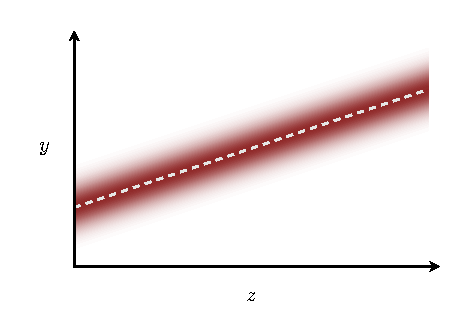
\includegraphics{figures/fidelity/precise_accurate/precise_accurate.pdf}

}

}

\subcaption{\label{fig-precise-accurate}}
\end{minipage}%
%
\begin{minipage}[t]{0.30\linewidth}

{\centering 

\raisebox{-\height}{

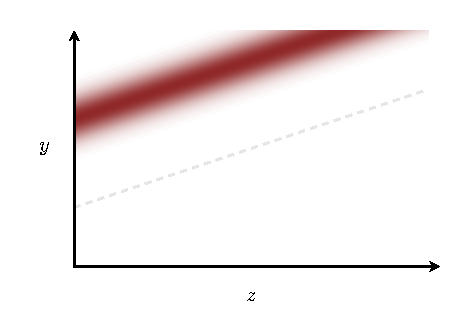
\includegraphics{figures/fidelity/precise_biased/precise_biased.pdf}

}

}

\subcaption{\label{fig-precise-biased}}
\end{minipage}%
%
\begin{minipage}[t]{0.30\linewidth}

{\centering 

\raisebox{-\height}{

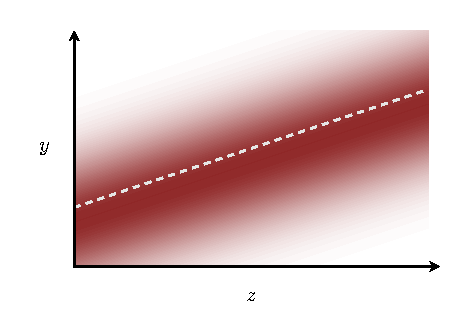
\includegraphics{figures/fidelity/imprecise/imprecise.pdf}

}

}

\subcaption{\label{fig-imprecise}}
\end{minipage}%
%
\begin{minipage}[t]{0.05\linewidth}

{\centering 

~

}

\end{minipage}%

\caption{\label{fig-fidelity}A fidelity model quantifies the
relationship between reviewer assessments \(y\) and the true latent
state \(z\). (a) In a precise and accurate fidelity model the
assessments concentrate around \(z\), making it straightforward to infer
the true latent state. (b) Precise but biased fidelity models correspond
to assessments that concentrate away from \(z\). If we can infer this
bias, however, we can still recover the true latent state. (c) An
imprecise fidelity model features little coupling between the
assessments and the latent state, making it difficult if not impossible
to infer the latent state.}

\end{figure}

Combining the reviewer fidelity models with a model \(\pi(z \mid \psi)\)
for the latent state defines a joint observational model over the latent
state and the individual assessments, \begin{align*}
\pi( y_{1}, \ldots, y_{R}, z \mid \phi_{1}, \ldots \phi_{R}, \psi)
&=
\pi( y_{1}, \ldots, y_{J} \mid z, \phi_{1}, \ldots \phi_{R}) \,
\pi( z \mid \psi )
\\
&=
\left[ \prod_{r = 1}^{R} \pi( y_{r} \mid z, \phi_{r}) \right] \,
\pi( z \mid \psi).
\end{align*} To ease the notation we can also write \begin{align*}
\mathbf{y} &= (y_{1}, \ldots, y_{R})
\\
\boldsymbol{\phi} &= (\phi_{1}, \ldots, \phi_{R})
\end{align*} with \[
\pi( \mathbf{y}, z \mid \boldsymbol{\phi}, \psi)
=
\left[ \prod_{r = 1}^{R} \pi( y_{r} \mid z, \phi_{r}) \right] \,
\pi( z \mid \psi).
\]

If the fidelity and latent state model configurations are fixed then a
collection of observed assessments, \[
\{ \tilde{y}_{1}, \ldots, \tilde{y}_{R} \},
\] allows us to infer an unknown latent state, \begin{align*}
\pi( z \mid \tilde{\mathbf{y}}, \boldsymbol{\phi}, \psi)
&\propto
\pi( \mathbf{y}, z \mid \boldsymbol{\phi}, \psi)
\\
&\propto
\left[ \prod_{r = 1}^{R} \pi( \tilde{y}_{r} \mid z, \phi_{r}) \right] \,
\pi( z \mid \psi).
\end{align*} Conceptually the reviewer consensus is given by the values
of \(z\) where the individual likelihood function contributions
\(\pi( \tilde{y}_{r} \mid z, \phi_{r})\) most strongly overlap (Figure
Figure~\ref{fig-inferential-consensus}).

\begin{figure}

{\centering 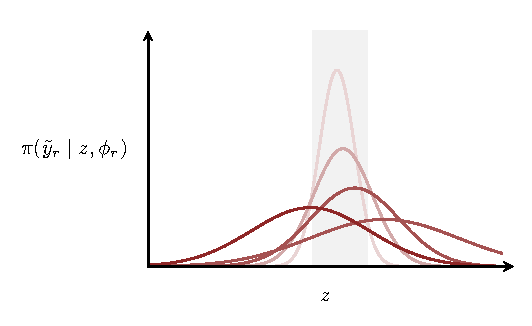
\includegraphics[width=0.75\textwidth,height=\textheight]{figures/inferential_consensus/inferential_consensus.pdf}

}

\caption{\label{fig-inferential-consensus}Evaluating the fidelity model
for each reviewer on an observed assessment gives a contribution to the
likelihood function, \(\pi( \tilde{y}_{r} \mid z, \phi_{r})\). The
overlap of these contributions defines the consensus of the reviewers.}

\end{figure}

When the fidelity and latent state model configurations are not known
but we have both a collection of observed assessments, \[
\{ \tilde{y}_{1}, \ldots, \tilde{y}_{R} \},
\] and a known latent state \(\tilde{z}\) the consensus model allows us
to infer these unknown parameters, \begin{align*}
\pi( \boldsymbol{\phi}, \psi \mid \tilde{z}, \tilde{\mathbf{y}} )
&\propto
\pi( \tilde{\mathbf{y}}, \tilde{z}, \boldsymbol{\phi}, \psi )
\\
&\propto
\pi( \tilde{\mathbf{y}}, \tilde{z} \mid \boldsymbol{\phi}, \psi ) \,
\pi( \boldsymbol{\phi}, \psi )
\\
&\propto
\left[ \prod_{r = 1}^{R}
       \pi( \tilde{y}_{r} \mid \tilde{z}, \phi_{r}) \right] \,
\pi( z \mid \psi) \, \pi( \boldsymbol{\phi}, \psi ).
\end{align*} In other words comparing reviewer responses to a known
truth allows us to \emph{calibrate} the accuracy of their assessments.

In the worst case the fidelity and latent state model configurations
will be unknown and we will have access to only the observed
assessments. Here we have to infer the model configurations and the
latent state at the same time, \begin{align*}
\pi( z, \boldsymbol{\phi}, \psi \mid \tilde{\mathbf{y}} )
&\propto
\pi( \tilde{\mathbf{y}}, z, \boldsymbol{\phi}, \psi)
\\
&\propto
\pi( \tilde{\mathbf{y}}, z \mid \boldsymbol{\phi}, \psi ) \,
\pi( \boldsymbol{\phi}, \psi )
\\
&\propto
\left[ \prod_{r = 1}^{R} \pi( \tilde{y}_{r} \mid z, \phi_{r}) \right] \,
\pi( z \mid \psi) \, \pi( \boldsymbol{\phi}, \psi ).
\end{align*}

Unfortunately these joint inferences are typically degenerate. For most
consensus models the observed assessments can be made manipulated into
consistent with \emph{any} latent state by configuring the individual
fidelity models appropriately.

Consider, for example, the \(Y = Z = \mathbb{R}\) and the fidelity
models \[
\pi( y_{r} | z, \mu, \tau_{j} )
=
\text{normal}( y_{r} | z + \mu, \tau_{j} ).
\] Observed assessments \(\tilde{y}_{r}\) will not directly inform the
latent state but rather the additive combination \(z + \mu\), and by
adjusting \(\mu\) the consensus can be shifted to any value of \(z\).

In most applications we will not be considering a single assessment but
rather a collection of \(N\) assessments. Not every reviewer has to
participate in every assessment, but if they do then the notation for
the joint model simplifies considerably, \[
\pi(\mathbf{y}_{1}, z_{1}, \ldots, \mathbf{y}_{N},
    \boldsymbol{\phi}, \psi)
=
\prod_{n = 1}^{N}
\prod_{r = 1}^{R} \pi( y_{nr} \mid z, \phi_{r}) \, \pi( z_{n} \mid \psi)
\pi(\boldsymbol{\phi}, \psi).
\]

In general these collections will have some combination of assessments
with and without accompanying observations of the true latent state. The
most complete observations \[
\{ \tilde{\mathbf{y}}_{n}, \tilde{z}_{n} \}
\] the more precisely we can infer the model configurations
\(\boldsymbol{\phi}\) and \(\psi\) and the more precisely we can infer
unobserved latent states for the incomplete observations.

Without complete observations we will need to find alternative ways to
suppress the degeneracies inherit to a particular consensus model. One
strategy that is always available is the incorporation of as much domain
expertise as possible in the prior model
\(\pi( \boldsymbol{\phi}, \psi )\). This approach will be limited,
however, by the domain expertise available for elicitation.

Another possibility is to integrate the consensus model with another
narratively generative model that quantifies observable consequences of
the latent state. In other words even if we can't observe the latent
state directly any indirect constraints through auxiliary observations
can help distinguish the reviewer fidelities from the true latent
states.

\hypertarget{finite-consensus-models}{%
\section{Finite Consensus Models}\label{finite-consensus-models}}

In general the assessments and latent states can take values in any
space. Often, however, the take values in finite spaces where any
consensus model takes on a particular form.

First let's assume that the latent state \(z\) can take one of only
\(K\) unordered values with the arbitrary labels
\(\{1, \ldots, k, \ldots, K \}\). In this case any latent state model
reduces to a collection of \(K\) probabilities, \[
\pi(z = k, \boldsymbol{\psi}) = \psi_{k}
\] with \[
0 \le \psi_{k} \le 1
\\
\sum_{k = 1}^{K} \psi_{k} = 1.
\] When the possible values are ordered then an
\href{https://betanalpha.github.io/assets/case_studies/ordinal_regression.html}{ordinal
model} is better equipped to accommodate neighboring correlations.

Although mathematically straightforward a discrete latent state
introduces a practical issue because we will not be able to use tools
like Hamiltonian Monte Carlo to quantify posterior inferences.
Fortunately we can work around this by marginalizing the discrete latent
state out of the joint observational model, \begin{align*}
\pi( \mathbf{y} \mid \boldsymbol{\phi}, \boldsymbol{\psi} )
&=
\sum_{k = 1}^{K} \pi( \mathbf{y}, k \mid
                      \boldsymbol{\phi}, \boldsymbol{\psi})
\\
&=
\sum_{k = 1}^{K} \prod_{r = 1}^{R} \pi( y_{r} \mid k, \phi_{r}) \,
                 \pi(k \mid \boldsymbol{\psi} )
\\
&=
\sum_{k = 1}^{K} \prod_{r = 1}^{R} \pi( y_{r} \mid k, \phi_{r}) \,
                 \psi_{k}
\\
&=
\sum_{k = 1}^{K} \psi_{k} \prod_{r = 1}^{R} \pi( y_{r} \mid k, \phi_{r}).
\end{align*}

In words the marginal observational model reduces to a mixture over the
possible latent states weighted by the simplex \(\boldsymbol{\psi}\).
Instead of trying to find a way to infer the discrete state \(z\) we can
use tools like Hamiltonian Monte Carlo to efficiently infer the
configuration of the continuous simplex \(\boldsymbol{\psi}\), and hence
how consistent each latent state configuration is with the observed
assessments.

When the assessments can take one of only \(J\) unordered values with
the arbitrary labels \(\{1, \ldots, j, \ldots, J \}\) then the fidelity
models similarly reduce to the probabilities \[
\pi( y_{r} = j \mid k, \boldsymbol{\phi}_{r}) = \phi_{r, jk}.
\] with \[
0 \le \phi_{r, jk} \le 1
\\
\sum_{j = 1}^{J} \gamma_{r, jk} = 1.
\] Once we restrict to finite, unordered spaces our models become
simplices all the way down.

Mathematically the collection of simplices that defines the fidelity
model for each reviewer can be organized into a matrix with one row for
each possible assessment outcome and one column for each possible latent
state configuration, \[
\Phi_{r} =
\left( \begin{array}{ccccc}
\phi_{r, 11} & \ldots & \phi_{r, 1k} & \ldots \phi_{r, 1K} \\
\ldots       & \ldots & \ldots       & \ldots              \\
\phi_{r, j1} & \ldots & \phi_{r, jk} & \ldots \phi_{r, jK} \\
\ldots       & \ldots & \ldots       & \ldots              \\
\phi_{r, J1} & \ldots & \phi_{r, Jk} & \ldots \phi_{r, JK} \\
\end{array} \right).
\] A matrix of probabilities where the elements across each column sum
to one like this is known as a \textbf{left stochastic matrix}, or
perhaps more appropriately \textbf{left probability matrix}.

This finite consensus model manifests a serious degeneracy. Any
permutation of the latent states, equivalently any relabeling of the
unordered values, can be compensated by permuting the columns of every
fidelity matrix without compromising the consistency with a given
observation. In other words a likelihood function informed by only
observed assessments, and not an observed latent state, will always
manifest \(K!\) separate modes, one for every one of the possible
permutations!

Often reviewers assess the latent state directly, instead of assessing
some indirectly consequence of the latent state. In this case we have
\(Y = Z\) and, in the finite setting, \(J = K\) so that every fidelity
matrix \(\Phi_{j}\) will be square.

If we believe that the reviewers are able to identify the true latent
state more often than not then we should have \[
\phi_{r, kk} > \phi_{r, kk'}
\] whenever \(k \ne k'\). In other words accurate reviewers are modeled
with diagonally dominant fidelity matrix.

Conveniently this constraint eliminates all but one of the peaks in the
realized likelihood functions. Unfortunately enforcing this constraint
in practice is not straightforward. Enforcing a hard constraint
\(\phi_{r, kk} > \phi_{r, kk'}\)r couples the column simplices together,
substantially complicating the viable fidelity matrix configurations. On
the other hand we can enforce a soft constraint with an informative
prior model over the column simplices, but this may not completely
eliminate the undesired modes.

That said neither a hard nor soft constraint is appropriate if the
reviewers are not necessarily expected to perform well. When our best
inferences are given by doing the exact opposite of what a reviewer
suggests then we'll need to consider other modes of the realized
likelihood functions.

Finite consensus models with \[
Y = Z = \{ 1, \ldots, K \}
\] are commonly known as \textbf{Dawid-Skene} models after Dawid and
Skene (1979), although the methodology was common earlier. See for
example Landis and Koch (1977). The problem of estimating the agreement
between multiple assessments has an even longer history; see for example
Good and Card (1971), Landis and Koch (1975a) and Landis and Koch
(1975b).

Regardless of the structure of the latent state space and the reviewer
assessment space I prefer to use the more general term ``consensus
modeling'' to emphasize the common construction shared by these models.

\hypertarget{demonstration}{%
\section{Demonstration}\label{demonstration}}

Let's see how all of these ideas are implemented in practice by drawing
inferences from a finite consensus model.

\hypertarget{set-up}{%
\subsection{Set Up}\label{set-up}}

First we set up our local \texttt{R} environment.

\begin{Shaded}
\begin{Highlighting}[]
\FunctionTok{par}\NormalTok{(}\AttributeTok{family=}\StringTok{"serif"}\NormalTok{, }\AttributeTok{las=}\DecValTok{1}\NormalTok{, }\AttributeTok{bty=}\StringTok{"l"}\NormalTok{,}
    \AttributeTok{cex.axis=}\DecValTok{1}\NormalTok{, }\AttributeTok{cex.lab=}\DecValTok{1}\NormalTok{, }\AttributeTok{cex.main=}\DecValTok{1}\NormalTok{,}
    \AttributeTok{xaxs=}\StringTok{"i"}\NormalTok{, }\AttributeTok{yaxs=}\StringTok{"i"}\NormalTok{, }\AttributeTok{mar =} \FunctionTok{c}\NormalTok{(}\DecValTok{5}\NormalTok{, }\DecValTok{5}\NormalTok{, }\DecValTok{3}\NormalTok{, }\DecValTok{5}\NormalTok{))}

\NormalTok{c\_light }\OtherTok{\textless{}{-}} \FunctionTok{c}\NormalTok{(}\StringTok{"\#DCBCBC"}\NormalTok{)}
\NormalTok{c\_light\_highlight }\OtherTok{\textless{}{-}} \FunctionTok{c}\NormalTok{(}\StringTok{"\#C79999"}\NormalTok{)}
\NormalTok{c\_mid }\OtherTok{\textless{}{-}} \FunctionTok{c}\NormalTok{(}\StringTok{"\#B97C7C"}\NormalTok{)}
\NormalTok{c\_mid\_highlight }\OtherTok{\textless{}{-}} \FunctionTok{c}\NormalTok{(}\StringTok{"\#A25050"}\NormalTok{)}
\NormalTok{c\_dark }\OtherTok{\textless{}{-}} \FunctionTok{c}\NormalTok{(}\StringTok{"\#8F2727"}\NormalTok{)}
\NormalTok{c\_dark\_highlight }\OtherTok{\textless{}{-}} \FunctionTok{c}\NormalTok{(}\StringTok{"\#7C0000"}\NormalTok{)}

\NormalTok{c\_light\_teal }\OtherTok{\textless{}{-}} \FunctionTok{c}\NormalTok{(}\StringTok{"\#6B8E8E"}\NormalTok{)}
\NormalTok{c\_mid\_teal }\OtherTok{\textless{}{-}} \FunctionTok{c}\NormalTok{(}\StringTok{"\#487575"}\NormalTok{)}
\NormalTok{c\_dark\_teal }\OtherTok{\textless{}{-}} \FunctionTok{c}\NormalTok{(}\StringTok{"\#1D4F4F"}\NormalTok{)}
\end{Highlighting}
\end{Shaded}

Then we load \texttt{RStan} and my recommended diagnostic suite.

\begin{Shaded}
\begin{Highlighting}[]
\FunctionTok{library}\NormalTok{(rstan)}
\FunctionTok{rstan\_options}\NormalTok{(}\AttributeTok{auto\_write =} \ConstantTok{TRUE}\NormalTok{)            }\CommentTok{\# Cache compiled Stan programs}
\FunctionTok{options}\NormalTok{(}\AttributeTok{mc.cores =}\NormalTok{ parallel}\SpecialCharTok{::}\FunctionTok{detectCores}\NormalTok{()) }\CommentTok{\# Parallelize chains}
\NormalTok{parallel}\SpecialCharTok{:::}\FunctionTok{setDefaultClusterOptions}\NormalTok{(}\AttributeTok{setup\_strategy =} \StringTok{"sequential"}\NormalTok{)}

\NormalTok{util }\OtherTok{\textless{}{-}} \FunctionTok{new.env}\NormalTok{()}
\FunctionTok{source}\NormalTok{(}\StringTok{\textquotesingle{}stan\_utility\_rstan.R\textquotesingle{}}\NormalTok{, }\AttributeTok{local=}\NormalTok{util)}
\end{Highlighting}
\end{Shaded}

\hypertarget{dirichlet-visualizations}{%
\subsection{Dirichlet Visualizations}\label{dirichlet-visualizations}}

Because we will be working with a finite consensus model we will be
employing a lot of simplices, one for the latent state in each
assessment and one for the responses of each reviewer given each of the
possible latent states. The most convenient prior models over the space
of simplices are given by the Dirichlet family of probability density
functions.

\begin{Shaded}
\begin{Highlighting}[]
\NormalTok{lmult }\OtherTok{\textless{}{-}} \ControlFlowTok{function}\NormalTok{(x, a) \{}
  \ControlFlowTok{if}\NormalTok{ (a }\SpecialCharTok{==} \DecValTok{0}\NormalTok{) \{}
\NormalTok{    (}\DecValTok{0}\NormalTok{)}
\NormalTok{  \} }\ControlFlowTok{else}\NormalTok{ \{}
\NormalTok{    (a }\SpecialCharTok{*} \FunctionTok{log}\NormalTok{(x))}
\NormalTok{  \}}
\NormalTok{\}}

\NormalTok{dirichlet\_pdf }\OtherTok{\textless{}{-}} \ControlFlowTok{function}\NormalTok{(p1, p2, p3, a1, a2, a3) \{}
  \FunctionTok{exp}\NormalTok{(  }\FunctionTok{lmult}\NormalTok{(p1, a1 }\SpecialCharTok{{-}} \DecValTok{1}\NormalTok{) }\SpecialCharTok{+} \FunctionTok{lmult}\NormalTok{(p2, a2 }\SpecialCharTok{{-}} \DecValTok{1}\NormalTok{) }\SpecialCharTok{+} \FunctionTok{lmult}\NormalTok{(p3, a3 }\SpecialCharTok{{-}} \DecValTok{1}\NormalTok{)}
      \SpecialCharTok{+} \FunctionTok{lgamma}\NormalTok{(a1 }\SpecialCharTok{+}\NormalTok{ a2 }\SpecialCharTok{+}\NormalTok{ a3) }\SpecialCharTok{{-}} \FunctionTok{lgamma}\NormalTok{(a1) }\SpecialCharTok{{-}} \FunctionTok{lgamma}\NormalTok{(a2) }\SpecialCharTok{{-}} \FunctionTok{lgamma}\NormalTok{(a3) )}
\NormalTok{\}}
\end{Highlighting}
\end{Shaded}

Conveniently we can completely visualize three-dimensional simplices,
and density functions over the possible simplex configurations, in a
two-dimensional plots that places the extreme states \[
(1, 0, 0), (0, 1, 0), (0, 0, 1)
\] at the corners of a triangle.

\begin{Shaded}
\begin{Highlighting}[]
\NormalTok{disc\_colors }\OtherTok{\textless{}{-}} \FunctionTok{c}\NormalTok{(}\StringTok{"\#FFFFFF"}\NormalTok{, }\StringTok{"\#DCBCBC"}\NormalTok{, }\StringTok{"\#C79999"}\NormalTok{, }\StringTok{"\#B97C7C"}\NormalTok{,}
                 \StringTok{"\#A25050"}\NormalTok{, }\StringTok{"\#8F2727"}\NormalTok{, }\StringTok{"\#7C0000"}\NormalTok{)}
\NormalTok{cont\_colors }\OtherTok{\textless{}{-}} \FunctionTok{colormap}\NormalTok{(}\AttributeTok{colormap=}\NormalTok{disc\_colors, }\AttributeTok{nshades=}\DecValTok{100}\NormalTok{)}

\NormalTok{plot\_dirichlet }\OtherTok{\textless{}{-}} \ControlFlowTok{function}\NormalTok{(a1, a2, a3, }\AttributeTok{label\_cex=}\DecValTok{1}\NormalTok{, }\AttributeTok{main\_title=}\ConstantTok{NA}\NormalTok{) \{}
\NormalTok{  N }\OtherTok{\textless{}{-}} \DecValTok{200}
\NormalTok{  C }\OtherTok{\textless{}{-}} \DecValTok{1} \SpecialCharTok{/} \FunctionTok{sqrt}\NormalTok{(}\DecValTok{3}\NormalTok{)}
\NormalTok{  xs }\OtherTok{\textless{}{-}} \FunctionTok{seq}\NormalTok{(}\SpecialCharTok{{-}}\NormalTok{C }\SpecialCharTok{{-}} \FloatTok{0.2}\NormalTok{, C }\SpecialCharTok{+} \FloatTok{0.2}\NormalTok{, (}\DecValTok{2} \SpecialCharTok{*}\NormalTok{ C }\SpecialCharTok{+} \FloatTok{0.4}\NormalTok{) }\SpecialCharTok{/}\NormalTok{ (N }\SpecialCharTok{{-}} \DecValTok{1}\NormalTok{))}
\NormalTok{  ys }\OtherTok{\textless{}{-}} \FunctionTok{seq}\NormalTok{(}\DecValTok{0} \SpecialCharTok{{-}} \FloatTok{0.1}\NormalTok{, }\DecValTok{1} \SpecialCharTok{+} \FloatTok{0.1}\NormalTok{, }\FloatTok{1.2} \SpecialCharTok{/}\NormalTok{ (N }\SpecialCharTok{{-}} \DecValTok{1}\NormalTok{))}
\NormalTok{  zs }\OtherTok{\textless{}{-}} \FunctionTok{matrix}\NormalTok{(}\DecValTok{0}\NormalTok{, }\AttributeTok{nrow=}\NormalTok{N, }\AttributeTok{ncol=}\NormalTok{N)}

  \ControlFlowTok{for}\NormalTok{ (n }\ControlFlowTok{in} \DecValTok{1}\SpecialCharTok{:}\NormalTok{N) \{}
    \ControlFlowTok{for}\NormalTok{ (m }\ControlFlowTok{in} \DecValTok{1}\SpecialCharTok{:}\NormalTok{N) \{}
\NormalTok{      p3 }\OtherTok{\textless{}{-}}\NormalTok{ ys[m]}
\NormalTok{      p2 }\OtherTok{\textless{}{-}}\NormalTok{ (}\DecValTok{1} \SpecialCharTok{+}\NormalTok{ xs[n] }\SpecialCharTok{/}\NormalTok{ C }\SpecialCharTok{{-}}\NormalTok{ ys[m]) }\SpecialCharTok{/} \DecValTok{2}
\NormalTok{      p1 }\OtherTok{\textless{}{-}}\NormalTok{ (}\DecValTok{1} \SpecialCharTok{{-}}\NormalTok{ xs[n] }\SpecialCharTok{/}\NormalTok{ C }\SpecialCharTok{{-}}\NormalTok{ ys[m]) }\SpecialCharTok{/} \DecValTok{2}
  
      \ControlFlowTok{if}\NormalTok{ (p1 }\SpecialCharTok{\textgreater{}=} \DecValTok{0} \SpecialCharTok{\&}\NormalTok{ p2 }\SpecialCharTok{\textgreater{}=} \DecValTok{0} \SpecialCharTok{\&}\NormalTok{ p3 }\SpecialCharTok{\textgreater{}=} \DecValTok{0} \SpecialCharTok{\&}\NormalTok{ p1 }\SpecialCharTok{+}\NormalTok{ p2 }\SpecialCharTok{+}\NormalTok{ p3 }\SpecialCharTok{\textless{}=} \DecValTok{1}\NormalTok{) \{}
\NormalTok{        zs[n, m] }\OtherTok{\textless{}{-}} \FunctionTok{dirichlet\_pdf}\NormalTok{(p1, p2, p3, a1, a2, a3)}
\NormalTok{      \} }\ControlFlowTok{else}\NormalTok{ \{}
\NormalTok{        zs[n, m] }\OtherTok{\textless{}{-}} \ConstantTok{NA}
\NormalTok{      \}}
\NormalTok{    \}}
\NormalTok{  \}}

  \ControlFlowTok{if}\NormalTok{ (}\FunctionTok{is.na}\NormalTok{(main\_title)) \{}
    \FunctionTok{par}\NormalTok{(}\AttributeTok{mar =} \FunctionTok{c}\NormalTok{(}\DecValTok{0}\NormalTok{, }\DecValTok{0}\NormalTok{, }\DecValTok{0}\NormalTok{, }\DecValTok{0}\NormalTok{))}
    \FunctionTok{image}\NormalTok{(xs, ys, zs, }\AttributeTok{col=}\FunctionTok{rev}\NormalTok{(cont\_colors), }\AttributeTok{axes=}\ConstantTok{FALSE}\NormalTok{, }\AttributeTok{ann=}\ConstantTok{FALSE}\NormalTok{)}
\NormalTok{  \} }\ControlFlowTok{else}\NormalTok{ \{}
    \FunctionTok{par}\NormalTok{(}\AttributeTok{mar =} \FunctionTok{c}\NormalTok{(}\DecValTok{0}\NormalTok{, }\DecValTok{0}\NormalTok{, }\DecValTok{1}\NormalTok{, }\DecValTok{0}\NormalTok{))}
    \FunctionTok{image}\NormalTok{(xs, ys, zs, }\AttributeTok{col=}\FunctionTok{rev}\NormalTok{(cont\_colors), }\AttributeTok{axes=}\ConstantTok{FALSE}\NormalTok{, }\AttributeTok{ann=}\ConstantTok{FALSE}\NormalTok{)}
    \FunctionTok{title}\NormalTok{(main\_title)}
\NormalTok{  \}}

  \FunctionTok{lines}\NormalTok{( }\FunctionTok{c}\NormalTok{(}\SpecialCharTok{{-}}\NormalTok{C, }\DecValTok{0}\NormalTok{), }\FunctionTok{c}\NormalTok{(}\DecValTok{0}\NormalTok{, }\DecValTok{1}\NormalTok{), }\AttributeTok{lwd=}\DecValTok{3}\NormalTok{)}
  \FunctionTok{lines}\NormalTok{( }\FunctionTok{c}\NormalTok{(}\SpecialCharTok{+}\NormalTok{C, }\DecValTok{0}\NormalTok{), }\FunctionTok{c}\NormalTok{(}\DecValTok{0}\NormalTok{, }\DecValTok{1}\NormalTok{), }\AttributeTok{lwd=}\DecValTok{3}\NormalTok{)}
  \FunctionTok{lines}\NormalTok{( }\FunctionTok{c}\NormalTok{(}\SpecialCharTok{{-}}\NormalTok{C, }\SpecialCharTok{+}\NormalTok{C), }\FunctionTok{c}\NormalTok{(}\DecValTok{0}\NormalTok{, }\DecValTok{0}\NormalTok{), }\AttributeTok{lwd=}\DecValTok{3}\NormalTok{)}

\NormalTok{  text\_delta }\OtherTok{\textless{}{-}} \FloatTok{0.05}
  \FunctionTok{text}\NormalTok{( }\DecValTok{0}\NormalTok{, }\DecValTok{1} \SpecialCharTok{+}\NormalTok{ text\_delta, }\StringTok{"(0, 0, 1)"}\NormalTok{, }\AttributeTok{cex=}\NormalTok{label\_cex)}
  \FunctionTok{text}\NormalTok{(}\SpecialCharTok{{-}}\NormalTok{C }\SpecialCharTok{{-}}\NormalTok{ text\_delta, }\SpecialCharTok{{-}}\NormalTok{text\_delta, }\StringTok{"(1, 0, 0)"}\NormalTok{, }\AttributeTok{cex=}\NormalTok{label\_cex)}
  \FunctionTok{text}\NormalTok{(}\SpecialCharTok{+}\NormalTok{C }\SpecialCharTok{+}\NormalTok{ text\_delta, }\SpecialCharTok{{-}}\NormalTok{text\_delta, }\StringTok{"(0, 1, 0)"}\NormalTok{, }\AttributeTok{cex=}\NormalTok{label\_cex)}

\NormalTok{  tick\_delta }\OtherTok{\textless{}{-}} \FloatTok{0.025}
  \FunctionTok{lines}\NormalTok{( }\FunctionTok{c}\NormalTok{(}\DecValTok{0}\NormalTok{, }\DecValTok{0}\NormalTok{), }\FunctionTok{c}\NormalTok{(}\DecValTok{0}\NormalTok{, tick\_delta), }\AttributeTok{lwd=}\DecValTok{3}\NormalTok{)}
  \FunctionTok{text}\NormalTok{(}\DecValTok{0}\NormalTok{, }\DecValTok{0} \SpecialCharTok{{-}}\NormalTok{ text\_delta, }\StringTok{"(1/2, 1/2, 0)"}\NormalTok{, }\AttributeTok{cex=}\NormalTok{label\_cex)}

  \FunctionTok{lines}\NormalTok{( }\FunctionTok{c}\NormalTok{(}\SpecialCharTok{+}\NormalTok{C }\SpecialCharTok{*} \FloatTok{0.5}\NormalTok{, }\SpecialCharTok{+}\NormalTok{C }\SpecialCharTok{*} \FloatTok{0.5} \SpecialCharTok{{-}}\NormalTok{ tick\_delta }\SpecialCharTok{*} \FloatTok{0.5} \SpecialCharTok{*} \FunctionTok{sqrt}\NormalTok{(}\DecValTok{3}\NormalTok{)),}
         \FunctionTok{c}\NormalTok{(}\FloatTok{0.5}\NormalTok{, }\FloatTok{0.5} \SpecialCharTok{{-}}\NormalTok{ tick\_delta }\SpecialCharTok{*} \FloatTok{0.5}\NormalTok{), }\AttributeTok{lwd=}\DecValTok{3}\NormalTok{)}
  \FunctionTok{text}\NormalTok{(C }\SpecialCharTok{*} \FloatTok{0.5} \SpecialCharTok{+}\NormalTok{ text\_delta }\SpecialCharTok{*} \FloatTok{0.5} \SpecialCharTok{*} \FunctionTok{sqrt}\NormalTok{(}\DecValTok{3}\NormalTok{) }\SpecialCharTok{+} \FloatTok{2.5} \SpecialCharTok{*}\NormalTok{ text\_delta,}
       \FloatTok{0.5} \SpecialCharTok{+}\NormalTok{ text\_delta }\SpecialCharTok{*} \FloatTok{0.5}\NormalTok{, }\StringTok{"(0, 1/2, 1/2)"}\NormalTok{, }\AttributeTok{cex=}\NormalTok{label\_cex)}

  \FunctionTok{lines}\NormalTok{( }\FunctionTok{c}\NormalTok{(}\SpecialCharTok{{-}}\NormalTok{C }\SpecialCharTok{*} \FloatTok{0.5}\NormalTok{, }\SpecialCharTok{{-}}\NormalTok{C }\SpecialCharTok{*} \FloatTok{0.5} \SpecialCharTok{+}\NormalTok{ tick\_delta }\SpecialCharTok{*} \FloatTok{0.5} \SpecialCharTok{*} \FunctionTok{sqrt}\NormalTok{(}\DecValTok{3}\NormalTok{)),}
         \FunctionTok{c}\NormalTok{(}\FloatTok{0.5}\NormalTok{, }\FloatTok{0.5} \SpecialCharTok{{-}}\NormalTok{ tick\_delta }\SpecialCharTok{*} \FloatTok{0.5}\NormalTok{), }\AttributeTok{lwd=}\DecValTok{3}\NormalTok{)}
  \FunctionTok{text}\NormalTok{(}\SpecialCharTok{{-}}\NormalTok{C }\SpecialCharTok{*} \FloatTok{0.5} \SpecialCharTok{{-}}\NormalTok{ text\_delta }\SpecialCharTok{*} \FloatTok{0.5} \SpecialCharTok{*} \FunctionTok{sqrt}\NormalTok{(}\DecValTok{3}\NormalTok{) }\SpecialCharTok{{-}} \FloatTok{2.5} \SpecialCharTok{*}\NormalTok{ text\_delta,}
       \FloatTok{0.5} \SpecialCharTok{+}\NormalTok{ text\_delta }\SpecialCharTok{*} \FloatTok{0.5}\NormalTok{, }\StringTok{"(1/2, 0, 1/2)"}\NormalTok{, }\AttributeTok{cex=}\NormalTok{label\_cex)}

  \FunctionTok{points}\NormalTok{(}\DecValTok{0}\NormalTok{, }\DecValTok{1}\SpecialCharTok{/}\DecValTok{3}\NormalTok{, }\AttributeTok{col=}\StringTok{"white"}\NormalTok{, }\AttributeTok{pch=}\DecValTok{16}\NormalTok{, }\AttributeTok{cex=}\FloatTok{1.5}\NormalTok{)}
  \FunctionTok{points}\NormalTok{(}\DecValTok{0}\NormalTok{, }\DecValTok{1}\SpecialCharTok{/}\DecValTok{3}\NormalTok{, }\AttributeTok{col=}\StringTok{"black"}\NormalTok{, }\AttributeTok{pch=}\DecValTok{16}\NormalTok{, }\AttributeTok{cex=}\DecValTok{1}\NormalTok{)}
  \FunctionTok{text}\NormalTok{(}\DecValTok{0}\NormalTok{, }\DecValTok{1}\SpecialCharTok{/}\DecValTok{3} \SpecialCharTok{{-}} \FloatTok{1.5} \SpecialCharTok{*}\NormalTok{ text\_delta, }\StringTok{"(1/3, 1/3, 1/3)"}\NormalTok{, }\AttributeTok{cex=}\NormalTok{label\_cex)}
\NormalTok{\}}
\end{Highlighting}
\end{Shaded}

One convenient way to interpret a Dirichlet probability density function
is to factor the parameters \(\alpha_{1}, \ldots, \alpha_{K}\) into a
\emph{template simplex} and a \emph{concentration parameter}, \[
( \alpha_{1}, \ldots, \alpha_{K} )
=
\tau \cdot ( \gamma_{1}, \ldots, \gamma_{K} ),
\] with \[
\sum_{k = 1}^{K} \gamma_{k} = 1.
\]

If \(\tau > 1\) then the implied probability distribution will
concentrate around the simplex configuration
\(\gamma_{1}, \ldots, \gamma_{K}\). The larger \(\tau\) is the stronger
this concentration will be.

On the other hand if \(\tau < 1\) then the implied probability
distribution will be repelled from the template simplex, concentrating
instead on the nearest simplex boundaries.

One exception is when any of the \(\alpha_{k}\) are equal to one. In
this case the Dirichlet probability density function will not depend on
the corresponding simplex component at all.

For example taking \[
\alpha_{1} = \ldots = \alpha_{k} = \ldots = \alpha_{K} = 1
\] defines a uniform probability density function across the simplex
configurations.

\begin{Shaded}
\begin{Highlighting}[]
\FunctionTok{plot\_dirichlet}\NormalTok{(}\DecValTok{1}\NormalTok{, }\DecValTok{1}\NormalTok{, }\DecValTok{1}\NormalTok{)}
\end{Highlighting}
\end{Shaded}

\begin{figure}[H]

{\centering \includegraphics{consensus_modeling_files/figure-pdf/unnamed-chunk-6-1.pdf}

}

\end{figure}

Increasing the parameters in the same way results in a probability
density function that concentrates around the equal probability
configuration.

\begin{Shaded}
\begin{Highlighting}[]
\FunctionTok{plot\_dirichlet}\NormalTok{(}\DecValTok{5}\NormalTok{, }\DecValTok{5}\NormalTok{, }\DecValTok{5}\NormalTok{)}
\end{Highlighting}
\end{Shaded}

\begin{figure}[H]

{\centering \includegraphics{consensus_modeling_files/figure-pdf/unnamed-chunk-7-1.pdf}

}

\end{figure}

Often domain expertise prefers one simplex component over the others.
Taking \(\alpha_{k} = 1\) and \(\alpha_{k' \ne k} < 1\) results in a
probability density function that concentrates around the configuration
where all probability is allocated to \(k\)th simplex component. As we
move away from this corner the Dirichlet probability density function
concentrates on the edges of the simplex.

\begin{Shaded}
\begin{Highlighting}[]
\FunctionTok{plot\_dirichlet}\NormalTok{(}\DecValTok{1}\NormalTok{, }\FloatTok{0.8}\NormalTok{, }\FloatTok{0.8}\NormalTok{)}
\end{Highlighting}
\end{Shaded}

\begin{figure}[H]

{\centering \includegraphics{consensus_modeling_files/figure-pdf/unnamed-chunk-8-1.pdf}

}

\end{figure}

If we instead take \(\alpha_{k} > 1\) and \(\alpha_{k' \ne k} = 1\)
gives probability density functions that also concentrate around the
same corner, but in this case the tails are uniform across the remaining
components.

\begin{Shaded}
\begin{Highlighting}[]
\FunctionTok{par}\NormalTok{(}\AttributeTok{mfrow=}\FunctionTok{c}\NormalTok{(}\DecValTok{2}\NormalTok{, }\DecValTok{2}\NormalTok{))}
\FunctionTok{plot\_dirichlet}\NormalTok{(}\DecValTok{2}\NormalTok{, }\DecValTok{1}\NormalTok{, }\DecValTok{1}\NormalTok{, }\FloatTok{0.75}\NormalTok{, }\StringTok{"alpha = (2, 1, 1)"}\NormalTok{)}
\FunctionTok{plot\_dirichlet}\NormalTok{(}\DecValTok{3}\NormalTok{, }\DecValTok{1}\NormalTok{, }\DecValTok{1}\NormalTok{, }\FloatTok{0.75}\NormalTok{, }\StringTok{"alpha = (3, 1, 1)"}\NormalTok{)}
\FunctionTok{plot\_dirichlet}\NormalTok{(}\DecValTok{4}\NormalTok{, }\DecValTok{1}\NormalTok{, }\DecValTok{1}\NormalTok{, }\FloatTok{0.75}\NormalTok{, }\StringTok{"alpha = (4, 1, 1)"}\NormalTok{)}
\FunctionTok{plot\_dirichlet}\NormalTok{(}\DecValTok{5}\NormalTok{, }\DecValTok{1}\NormalTok{, }\DecValTok{1}\NormalTok{, }\FloatTok{0.75}\NormalTok{, }\StringTok{"alpha = (5, 1, 1)"}\NormalTok{)}
\end{Highlighting}
\end{Shaded}

\begin{figure}[H]

{\centering \includegraphics{consensus_modeling_files/figure-pdf/unnamed-chunk-9-1.pdf}

}

\end{figure}

These latter probability density functions are particularly well-suited
to isolating a single mode from degenerate inferences common to finite
consensus models.

\hypertarget{simulate-data}{%
\subsection{Simulate Data}\label{simulate-data}}

Because of the generative structure of the consensus model simulating
data is straightforward. Note that these simulations will be somewhat
optimistic, assuming that the reviewer fidelities strongly concentrate
around the true latent states.

\begin{codelisting}

\caption{\texttt{simu.stan}}

\begin{Shaded}
\begin{Highlighting}[]
\KeywordTok{transformed data}\NormalTok{ \{}
  \DataTypeTok{int}\NormalTok{\textless{}}\KeywordTok{lower}\NormalTok{=}\DecValTok{0}\NormalTok{\textgreater{} K = }\DecValTok{3}\NormalTok{;}
  \DataTypeTok{int}\NormalTok{\textless{}}\KeywordTok{lower}\NormalTok{=}\DecValTok{0}\NormalTok{\textgreater{} N\_reviewers = }\DecValTok{5}\NormalTok{;}
  \DataTypeTok{int}\NormalTok{\textless{}}\KeywordTok{lower}\NormalTok{=}\DecValTok{0}\NormalTok{\textgreater{} N\_assessments = }\DecValTok{110}\NormalTok{;}
  
  \DataTypeTok{vector}\NormalTok{[K] psi = [ }\FloatTok{0.4}\NormalTok{, }\FloatTok{0.3}\NormalTok{, }\FloatTok{0.3}\NormalTok{ ]\textquotesingle{};}
  \DataTypeTok{vector}\NormalTok{[K] fidelity[N\_reviewers, K];}
  
  \ControlFlowTok{for}\NormalTok{ (r }\ControlFlowTok{in} \DecValTok{1}\NormalTok{:N\_reviewers) \{}
    \ControlFlowTok{for}\NormalTok{ (k }\ControlFlowTok{in} \DecValTok{1}\NormalTok{:K) \{}
      \DataTypeTok{vector}\NormalTok{[K] alpha = rep\_vector(}\DecValTok{1}\NormalTok{, K);}
\NormalTok{      alpha[k] = }\DecValTok{10}\NormalTok{;}
\NormalTok{      fidelity[r, k] = dirichlet\_rng(alpha);}
\NormalTok{    \}}
\NormalTok{  \}}
\NormalTok{\}}

\KeywordTok{generated quantities}\NormalTok{ \{}
  \DataTypeTok{int}\NormalTok{\textless{}}\KeywordTok{lower}\NormalTok{=}\DecValTok{0}\NormalTok{, }\KeywordTok{upper}\NormalTok{=K\textgreater{} z[N\_assessments];}
  \DataTypeTok{int}\NormalTok{\textless{}}\KeywordTok{lower}\NormalTok{=}\DecValTok{0}\NormalTok{, }\KeywordTok{upper}\NormalTok{=K\textgreater{} y[N\_assessments, N\_reviewers];}
  
  \ControlFlowTok{for}\NormalTok{ (n }\ControlFlowTok{in} \DecValTok{1}\NormalTok{:N\_assessments) \{}
\NormalTok{    z[n] = categorical\_rng(psi);}
    
    \ControlFlowTok{for}\NormalTok{ (r }\ControlFlowTok{in} \DecValTok{1}\NormalTok{:N\_reviewers) \{}
\NormalTok{      y[n, r] = categorical\_rng(fidelity[r, z[n]]);}
\NormalTok{    \}}
\NormalTok{  \}}
\NormalTok{\}}
\end{Highlighting}
\end{Shaded}

\end{codelisting}

\begin{Shaded}
\begin{Highlighting}[]
\NormalTok{simu }\OtherTok{\textless{}{-}} \FunctionTok{stan}\NormalTok{(}\AttributeTok{file=}\StringTok{"stan\_programs/simu.stan"}\NormalTok{,}
             \AttributeTok{iter=}\DecValTok{1}\NormalTok{, }\AttributeTok{warmup=}\DecValTok{0}\NormalTok{, }\AttributeTok{chains=}\DecValTok{1}\NormalTok{,}
             \AttributeTok{seed=}\DecValTok{4838282}\NormalTok{, }\AttributeTok{algorithm=}\StringTok{"Fixed\_param"}\NormalTok{)}
\end{Highlighting}
\end{Shaded}

\begin{verbatim}

SAMPLING FOR MODEL 'simu' NOW (CHAIN 1).
Chain 1: Iteration: 1 / 1 [100%]  (Sampling)
Chain 1: 
Chain 1:  Elapsed Time: 0 seconds (Warm-up)
Chain 1:                0.000199 seconds (Sampling)
Chain 1:                0.000199 seconds (Total)
Chain 1: 
\end{verbatim}

Let's isolate the first 100 assessments as our main data set.

\begin{Shaded}
\begin{Highlighting}[]
\NormalTok{data }\OtherTok{\textless{}{-}} \FunctionTok{list}\NormalTok{(}\StringTok{\textquotesingle{}K\textquotesingle{}} \OtherTok{=} \DecValTok{3}\NormalTok{, }\StringTok{\textquotesingle{}N\_reviewers\textquotesingle{}} \OtherTok{=} \DecValTok{5}\NormalTok{, }\StringTok{\textquotesingle{}N\_assessments\textquotesingle{}} \OtherTok{=} \DecValTok{100}\NormalTok{,}
             \StringTok{\textquotesingle{}y\textquotesingle{}} \OtherTok{=} \FunctionTok{extract}\NormalTok{(simu)}\SpecialCharTok{$}\NormalTok{y[}\DecValTok{1}\NormalTok{,}\DecValTok{1}\SpecialCharTok{:}\DecValTok{100}\NormalTok{,])}

\NormalTok{true\_zs }\OtherTok{\textless{}{-}} \FunctionTok{extract}\NormalTok{(simu)}\SpecialCharTok{$}\NormalTok{z[}\DecValTok{1}\NormalTok{,}\DecValTok{1}\SpecialCharTok{:}\DecValTok{100}\NormalTok{]}
\end{Highlighting}
\end{Shaded}

The last 10 assessments we'll reserve along with the true latent states
as a separate calibration data set.

\begin{Shaded}
\begin{Highlighting}[]
\NormalTok{calib\_data }\OtherTok{\textless{}{-}} \FunctionTok{list}\NormalTok{(}\StringTok{\textquotesingle{}N\_calib\_assessments\textquotesingle{}} \OtherTok{=} \DecValTok{10}\NormalTok{,}
                   \StringTok{\textquotesingle{}y\_calib\textquotesingle{}} \OtherTok{=} \FunctionTok{extract}\NormalTok{(simu)}\SpecialCharTok{$}\NormalTok{y[}\DecValTok{1}\NormalTok{,}\DecValTok{101}\SpecialCharTok{:}\DecValTok{110}\NormalTok{,],}
                   \StringTok{\textquotesingle{}z\_calib\textquotesingle{}} \OtherTok{=} \FunctionTok{extract}\NormalTok{(simu)}\SpecialCharTok{$}\NormalTok{z[}\DecValTok{1}\NormalTok{,}\DecValTok{101}\SpecialCharTok{:}\DecValTok{110}\NormalTok{])}
\end{Highlighting}
\end{Shaded}

\hypertarget{display-data}{%
\subsection{Display Data}\label{display-data}}

Before attempting a fit let's explore our data a bit.

A natural summary for each assessment is a histogram of the reviewer
responses.

\begin{Shaded}
\begin{Highlighting}[]
\NormalTok{plot\_line\_hist }\OtherTok{\textless{}{-}} \ControlFlowTok{function}\NormalTok{(s, bin\_min, bin\_max, delta,}
\NormalTok{                           xlab, }\AttributeTok{ylim=}\ConstantTok{NA}\NormalTok{, }\AttributeTok{main=}\StringTok{""}\NormalTok{) \{}
\NormalTok{  bins }\OtherTok{\textless{}{-}} \FunctionTok{seq}\NormalTok{(bin\_min, bin\_max, delta)}
\NormalTok{  B }\OtherTok{\textless{}{-}} \FunctionTok{length}\NormalTok{(bins) }\SpecialCharTok{{-}} \DecValTok{1}
\NormalTok{  idx }\OtherTok{\textless{}{-}} \FunctionTok{rep}\NormalTok{(}\DecValTok{1}\SpecialCharTok{:}\NormalTok{B, }\AttributeTok{each=}\DecValTok{2}\NormalTok{)}
\NormalTok{  x }\OtherTok{\textless{}{-}} \FunctionTok{sapply}\NormalTok{(}\DecValTok{1}\SpecialCharTok{:}\FunctionTok{length}\NormalTok{(idx),}
              \ControlFlowTok{function}\NormalTok{(b) }\ControlFlowTok{if}\NormalTok{(b }\SpecialCharTok{\%\%} \DecValTok{2} \SpecialCharTok{==} \DecValTok{1}\NormalTok{) bins[idx[b]]}
                          \ControlFlowTok{else}\NormalTok{            bins[idx[b] }\SpecialCharTok{+} \DecValTok{1}\NormalTok{])}
\NormalTok{  x }\OtherTok{\textless{}{-}} \FunctionTok{c}\NormalTok{(bin\_min }\SpecialCharTok{{-}} \DecValTok{10}\NormalTok{, x, bin\_max }\SpecialCharTok{+} \DecValTok{10}\NormalTok{)}

\NormalTok{  counts }\OtherTok{\textless{}{-}} \FunctionTok{hist}\NormalTok{(s, }\AttributeTok{breaks=}\NormalTok{bins, }\AttributeTok{plot=}\ConstantTok{FALSE}\NormalTok{)}\SpecialCharTok{$}\NormalTok{counts}
\NormalTok{  y }\OtherTok{\textless{}{-}}\NormalTok{ counts[idx]}
\NormalTok{  y }\OtherTok{\textless{}{-}} \FunctionTok{c}\NormalTok{(}\DecValTok{0}\NormalTok{, y, }\DecValTok{0}\NormalTok{)}

\NormalTok{  ymax }\OtherTok{\textless{}{-}} \FunctionTok{max}\NormalTok{(y) }\SpecialCharTok{+} \DecValTok{1}

  \ControlFlowTok{if}\NormalTok{ (}\FunctionTok{any}\NormalTok{(}\FunctionTok{is.na}\NormalTok{(ylim))) \{}
\NormalTok{    ylim }\OtherTok{\textless{}{-}} \FunctionTok{c}\NormalTok{(}\DecValTok{0}\NormalTok{, ymax)}
\NormalTok{  \}}

  \FunctionTok{plot}\NormalTok{(x, y, }\AttributeTok{type=}\StringTok{"l"}\NormalTok{, }\AttributeTok{main=}\NormalTok{main, }\AttributeTok{col=}\StringTok{"black"}\NormalTok{, }\AttributeTok{lwd=}\DecValTok{2}\NormalTok{,}
       \AttributeTok{xlab=}\NormalTok{xlab, }\AttributeTok{xlim=}\FunctionTok{c}\NormalTok{(bin\_min, bin\_max),}
       \AttributeTok{ylab=}\StringTok{"Counts"}\NormalTok{, }\AttributeTok{ylim=}\NormalTok{ylim)}
\NormalTok{\}}
\end{Highlighting}
\end{Shaded}

We won't look at every assessment here, but examining the first nine we
can see that, while there is often disagreement, the most common
reviewer response always seems to align with the true latent state.

\begin{Shaded}
\begin{Highlighting}[]
\FunctionTok{par}\NormalTok{(}\AttributeTok{mfrow=}\FunctionTok{c}\NormalTok{(}\DecValTok{3}\NormalTok{, }\DecValTok{3}\NormalTok{), }\AttributeTok{mar =} \FunctionTok{c}\NormalTok{(}\DecValTok{5}\NormalTok{, }\DecValTok{4}\NormalTok{, }\DecValTok{2}\NormalTok{, }\DecValTok{1}\NormalTok{))}

\ControlFlowTok{for}\NormalTok{ (n }\ControlFlowTok{in} \DecValTok{1}\SpecialCharTok{:}\DecValTok{9}\NormalTok{) \{}
  \FunctionTok{plot\_line\_hist}\NormalTok{(data}\SpecialCharTok{$}\NormalTok{y[n,], }\SpecialCharTok{{-}}\FloatTok{0.5}\NormalTok{, data}\SpecialCharTok{$}\NormalTok{K }\SpecialCharTok{+} \FloatTok{1.5}\NormalTok{, }\DecValTok{1}\NormalTok{, }\StringTok{"Answer"}\NormalTok{,}
                 \FunctionTok{c}\NormalTok{(}\DecValTok{0}\NormalTok{, }\FloatTok{5.5}\NormalTok{), }\FunctionTok{paste}\NormalTok{(}\StringTok{"Assessment"}\NormalTok{, n))}
  \FunctionTok{abline}\NormalTok{(}\AttributeTok{v=}\NormalTok{true\_zs[n], }\AttributeTok{lwd=}\DecValTok{3}\NormalTok{, }\AttributeTok{col=}\NormalTok{c\_light)}
\NormalTok{\}}
\end{Highlighting}
\end{Shaded}

\begin{figure}[H]

{\centering \includegraphics{consensus_modeling_files/figure-pdf/unnamed-chunk-14-1.pdf}

}

\end{figure}

This is consistent with the highly-optimistic accuracies encoded in our
simulation.

\hypertarget{model-1}{%
\subsection{Model 1}\label{model-1}}

Let's begin with a lazy elicitation of our domain expertise, defaulting
to uniform Dirichlet priors for all of the simplices in our model.

\begin{codelisting}

\caption{\texttt{fit1.stan}}

\begin{Shaded}
\begin{Highlighting}[]
\KeywordTok{data}\NormalTok{ \{}
  \DataTypeTok{int}\NormalTok{\textless{}}\KeywordTok{lower}\NormalTok{=}\DecValTok{0}\NormalTok{\textgreater{} K;}
  \DataTypeTok{int}\NormalTok{\textless{}}\KeywordTok{lower}\NormalTok{=}\DecValTok{0}\NormalTok{\textgreater{} N\_reviewers;}
  \DataTypeTok{int}\NormalTok{\textless{}}\KeywordTok{lower}\NormalTok{=}\DecValTok{0}\NormalTok{\textgreater{} N\_assessments;}

  \DataTypeTok{int}\NormalTok{\textless{}}\KeywordTok{lower}\NormalTok{=}\DecValTok{0}\NormalTok{, }\KeywordTok{upper}\NormalTok{=K\textgreater{} y[N\_assessments, N\_reviewers];}
\NormalTok{\}}

\KeywordTok{parameters}\NormalTok{ \{}
  \CommentTok{// One simplex for the true answers of every assessment}
  \DataTypeTok{simplex}\NormalTok{[K] psi[N\_assessments];}
  
  \CommentTok{// One simplex per reviewer per possible true answers}
  \DataTypeTok{simplex}\NormalTok{[K] fidelity[N\_reviewers, K];}
\NormalTok{\}}

\KeywordTok{model}\NormalTok{ \{}
  \ControlFlowTok{for}\NormalTok{ (n }\ControlFlowTok{in} \DecValTok{1}\NormalTok{:N\_assessments) \{}
\NormalTok{    psi[n] \textasciitilde{} dirichlet(rep\_vector(}\DecValTok{1}\NormalTok{, K));}
\NormalTok{  \}}
  
  \ControlFlowTok{for}\NormalTok{ (r }\ControlFlowTok{in} \DecValTok{1}\NormalTok{:N\_reviewers) \{}
    \ControlFlowTok{for}\NormalTok{ (k }\ControlFlowTok{in} \DecValTok{1}\NormalTok{:K) \{}
      \DataTypeTok{vector}\NormalTok{[K] alpha = rep\_vector(}\DecValTok{1}\NormalTok{, K);}
\NormalTok{      fidelity[r, k] \textasciitilde{} dirichlet(alpha);}
\NormalTok{    \}}
\NormalTok{  \}}
  
  \ControlFlowTok{for}\NormalTok{ (n }\ControlFlowTok{in} \DecValTok{1}\NormalTok{:N\_assessments) \{}
    \DataTypeTok{real}\NormalTok{ lds[K];}
    
    \CommentTok{// Loop over possible correct answers}
    \ControlFlowTok{for}\NormalTok{ (k }\ControlFlowTok{in} \DecValTok{1}\NormalTok{:K) \{}
\NormalTok{      lds[k] = psi[n][k]; }\CommentTok{// Probability of kth answer being correct }
      \ControlFlowTok{for}\NormalTok{ (r }\ControlFlowTok{in} \DecValTok{1}\NormalTok{:N\_reviewers) \{}
        \CommentTok{// Probability of response given that the kth answer is correct}
        \DataTypeTok{real}\NormalTok{ p\_response = fidelity[r, k][y[n, r]];}
\NormalTok{        lds[k] += log(p\_response);}
\NormalTok{      \}}
\NormalTok{    \}}
    \KeywordTok{target +=}\NormalTok{ log\_sum\_exp(lds);}
\NormalTok{  \}}
\NormalTok{\}}

\KeywordTok{generated quantities}\NormalTok{ \{}
  \DataTypeTok{int}\NormalTok{\textless{}}\KeywordTok{lower}\NormalTok{=}\DecValTok{0}\NormalTok{, }\KeywordTok{upper}\NormalTok{=K\textgreater{} y\_pred[N\_assessments, N\_reviewers];}
  \ControlFlowTok{for}\NormalTok{ (n }\ControlFlowTok{in} \DecValTok{1}\NormalTok{:N\_assessments) \{}
    \DataTypeTok{int}\NormalTok{ z = categorical\_rng(psi[n]);}
    \ControlFlowTok{for}\NormalTok{ (r }\ControlFlowTok{in} \DecValTok{1}\NormalTok{:N\_reviewers) \{}
\NormalTok{      y\_pred[n, r] = categorical\_rng(fidelity[r, z]);}
\NormalTok{    \}}
\NormalTok{  \}}
\NormalTok{\}}
\end{Highlighting}
\end{Shaded}

\end{codelisting}

\begin{Shaded}
\begin{Highlighting}[]
\NormalTok{fit }\OtherTok{\textless{}{-}} \FunctionTok{stan}\NormalTok{(}\AttributeTok{file=}\StringTok{"stan\_programs/fit1.stan"}\NormalTok{,}
            \AttributeTok{data=}\NormalTok{data, }\AttributeTok{seed=}\DecValTok{8438338}\NormalTok{,}
            \AttributeTok{warmup=}\DecValTok{1000}\NormalTok{, }\AttributeTok{iter=}\DecValTok{2024}\NormalTok{, }\AttributeTok{refresh=}\DecValTok{0}\NormalTok{)}
\end{Highlighting}
\end{Shaded}

The diagnostics are a torrent of split \(\hat{R}\) issues for the
reviewer fidelities parameters.

\begin{Shaded}
\begin{Highlighting}[]
\NormalTok{diagnostics }\OtherTok{\textless{}{-}}\NormalTok{ util}\SpecialCharTok{$}\FunctionTok{extract\_hmc\_diagnostics}\NormalTok{(fit)}
\NormalTok{util}\SpecialCharTok{$}\FunctionTok{check\_all\_hmc\_diagnostics}\NormalTok{(diagnostics)}
\end{Highlighting}
\end{Shaded}

\begin{verbatim}
  All Hamiltonian Monte Carlo diagnostics are consistent with reliable
Markov chain Monte Carlo.
\end{verbatim}

\begin{Shaded}
\begin{Highlighting}[]
\NormalTok{samples }\OtherTok{\textless{}{-}}\NormalTok{ util}\SpecialCharTok{$}\FunctionTok{extract\_expectands}\NormalTok{(fit)}
\NormalTok{names }\OtherTok{\textless{}{-}} \FunctionTok{grep}\NormalTok{(}\StringTok{\textquotesingle{}pred\textquotesingle{}}\NormalTok{, }\FunctionTok{names}\NormalTok{(samples), }\AttributeTok{value=}\ConstantTok{TRUE}\NormalTok{, }\AttributeTok{invert=}\ConstantTok{TRUE}\NormalTok{)}
\NormalTok{base\_samples }\OtherTok{\textless{}{-}}\NormalTok{ samples[names]}
\NormalTok{util}\SpecialCharTok{$}\FunctionTok{check\_all\_expectand\_diagnostics}\NormalTok{(base\_samples)}
\end{Highlighting}
\end{Shaded}

\begin{verbatim}
fidelity[1,1,1]:
  Split hat{R} (3.411) exceeds 1.1!

fidelity[2,1,1]:
  Split hat{R} (5.701) exceeds 1.1!

fidelity[3,1,1]:
  Split hat{R} (6.300) exceeds 1.1!

fidelity[4,1,1]:
  Split hat{R} (5.974) exceeds 1.1!

fidelity[5,1,1]:
  Split hat{R} (6.276) exceeds 1.1!

fidelity[2,2,1]:
  Split hat{R} (1.453) exceeds 1.1!

fidelity[4,2,1]:
  Split hat{R} (1.561) exceeds 1.1!

fidelity[5,2,1]:
  Split hat{R} (1.175) exceeds 1.1!

fidelity[1,3,1]:
  Split hat{R} (4.294) exceeds 1.1!

fidelity[2,3,1]:
  Split hat{R} (6.106) exceeds 1.1!

fidelity[3,3,1]:
  Split hat{R} (8.200) exceeds 1.1!

fidelity[4,3,1]:
  Split hat{R} (6.682) exceeds 1.1!

fidelity[5,3,1]:
  Split hat{R} (5.408) exceeds 1.1!

fidelity[1,1,2]:
  Split hat{R} (5.586) exceeds 1.1!

fidelity[2,1,2]:
  Split hat{R} (6.775) exceeds 1.1!

fidelity[3,1,2]:
  Split hat{R} (6.517) exceeds 1.1!

fidelity[4,1,2]:
  Split hat{R} (4.204) exceeds 1.1!

fidelity[5,1,2]:
  Split hat{R} (5.952) exceeds 1.1!

fidelity[1,2,2]:
  Split hat{R} (6.120) exceeds 1.1!

fidelity[2,2,2]:
  Split hat{R} (5.380) exceeds 1.1!

fidelity[3,2,2]:
  Split hat{R} (7.309) exceeds 1.1!

fidelity[4,2,2]:
  Split hat{R} (3.141) exceeds 1.1!

fidelity[5,2,2]:
  Split hat{R} (5.723) exceeds 1.1!

fidelity[1,3,2]:
  Split hat{R} (6.719) exceeds 1.1!

fidelity[2,3,2]:
  Split hat{R} (6.158) exceeds 1.1!

fidelity[3,3,2]:
  Split hat{R} (7.135) exceeds 1.1!

fidelity[4,3,2]:
  Split hat{R} (5.094) exceeds 1.1!

fidelity[5,3,2]:
  Split hat{R} (5.489) exceeds 1.1!

fidelity[1,1,3]:
  Split hat{R} (5.066) exceeds 1.1!

fidelity[2,1,3]:
  Split hat{R} (5.372) exceeds 1.1!

fidelity[3,1,3]:
  Split hat{R} (7.116) exceeds 1.1!

fidelity[4,1,3]:
  Split hat{R} (2.741) exceeds 1.1!

fidelity[5,1,3]:
  Split hat{R} (6.576) exceeds 1.1!

fidelity[1,2,3]:
  Split hat{R} (4.109) exceeds 1.1!

fidelity[2,2,3]:
  Split hat{R} (3.631) exceeds 1.1!

fidelity[3,2,3]:
  Split hat{R} (5.696) exceeds 1.1!

fidelity[4,2,3]:
  Split hat{R} (2.195) exceeds 1.1!

fidelity[5,2,3]:
  Split hat{R} (6.132) exceeds 1.1!

fidelity[1,3,3]:
  Split hat{R} (1.525) exceeds 1.1!

fidelity[3,3,3]:
  Split hat{R} (1.330) exceeds 1.1!

fidelity[4,3,3]:
  Split hat{R} (1.466) exceeds 1.1!


Split Rhat larger than 1.1 suggests that at least one of the Markov
chains has not reached an equilibrium.
\end{verbatim}

Because we don't see accompanying empirical effective sample size
warnings the most likely culprit is multimodality in the posterior
distribution.

Before exploring for any multimodality, however, let's examine the
posterior retrodicive performance. We'll use the histogram of reviewer
responses for each assessment as our summary statistics.

\begin{Shaded}
\begin{Highlighting}[]
\NormalTok{hist\_retro }\OtherTok{\textless{}{-}} \ControlFlowTok{function}\NormalTok{(obs, samples, pred\_names,}
\NormalTok{                       bin\_min, bin\_max, delta,}
                       \AttributeTok{xlab=}\StringTok{""}\NormalTok{, }\AttributeTok{ylim=}\ConstantTok{NA}\NormalTok{, }\AttributeTok{title=}\StringTok{""}\NormalTok{) \{}
  \ControlFlowTok{if}\NormalTok{ (}\FunctionTok{is.na}\NormalTok{(bin\_min)) bin\_min }\OtherTok{\textless{}{-}} \FunctionTok{min}\NormalTok{(pred)}
  \ControlFlowTok{if}\NormalTok{ (}\FunctionTok{is.na}\NormalTok{(bin\_max)) bin\_max }\OtherTok{\textless{}{-}} \FunctionTok{max}\NormalTok{(pred)}
\NormalTok{  breaks }\OtherTok{\textless{}{-}} \FunctionTok{seq}\NormalTok{(bin\_min, bin\_max, delta)}
\NormalTok{  B }\OtherTok{\textless{}{-}} \FunctionTok{length}\NormalTok{(breaks) }\SpecialCharTok{{-}} \DecValTok{1}

\NormalTok{  idx }\OtherTok{\textless{}{-}} \FunctionTok{rep}\NormalTok{(}\DecValTok{1}\SpecialCharTok{:}\NormalTok{B, }\AttributeTok{each=}\DecValTok{2}\NormalTok{)}
\NormalTok{  xs }\OtherTok{\textless{}{-}} \FunctionTok{sapply}\NormalTok{(}\DecValTok{1}\SpecialCharTok{:}\FunctionTok{length}\NormalTok{(idx),}
               \ControlFlowTok{function}\NormalTok{(b) }\ControlFlowTok{if}\NormalTok{(b }\SpecialCharTok{\%\%} \DecValTok{2} \SpecialCharTok{==} \DecValTok{0}\NormalTok{) breaks[idx[b] }\SpecialCharTok{+} \DecValTok{1}\NormalTok{]}
                           \ControlFlowTok{else}\NormalTok{            breaks[idx[b]] )}

\NormalTok{  obs\_counts }\OtherTok{\textless{}{-}} \FunctionTok{hist}\NormalTok{(obs, }\AttributeTok{breaks=}\NormalTok{breaks, }\AttributeTok{plot=}\ConstantTok{FALSE}\NormalTok{)}\SpecialCharTok{$}\NormalTok{counts}
\NormalTok{  pad\_obs\_counts }\OtherTok{\textless{}{-}} \FunctionTok{do.call}\NormalTok{(cbind,}
                            \FunctionTok{lapply}\NormalTok{(idx, }\ControlFlowTok{function}\NormalTok{(n) obs\_counts[n]))}

\NormalTok{  pred }\OtherTok{\textless{}{-}} \FunctionTok{sapply}\NormalTok{(pred\_names,}
                 \ControlFlowTok{function}\NormalTok{(name) }\FunctionTok{c}\NormalTok{(}\FunctionTok{t}\NormalTok{(samples[[name]]), }\AttributeTok{recursive=}\ConstantTok{TRUE}\NormalTok{))}
\NormalTok{  N }\OtherTok{\textless{}{-}} \FunctionTok{dim}\NormalTok{(pred)[}\DecValTok{1}\NormalTok{]}
\NormalTok{  pred\_counts }\OtherTok{\textless{}{-}} \FunctionTok{sapply}\NormalTok{(}\DecValTok{1}\SpecialCharTok{:}\NormalTok{N,}
                        \ControlFlowTok{function}\NormalTok{(n) }\FunctionTok{hist}\NormalTok{(pred[n,],}
                                         \AttributeTok{breaks=}\NormalTok{breaks,}
                                         \AttributeTok{plot=}\ConstantTok{FALSE}\NormalTok{)}\SpecialCharTok{$}\NormalTok{counts)}

\NormalTok{  probs }\OtherTok{=} \FunctionTok{c}\NormalTok{(}\FloatTok{0.1}\NormalTok{, }\FloatTok{0.2}\NormalTok{, }\FloatTok{0.3}\NormalTok{, }\FloatTok{0.4}\NormalTok{, }\FloatTok{0.5}\NormalTok{, }\FloatTok{0.6}\NormalTok{, }\FloatTok{0.7}\NormalTok{, }\FloatTok{0.8}\NormalTok{, }\FloatTok{0.9}\NormalTok{)}
\NormalTok{  cred }\OtherTok{\textless{}{-}} \FunctionTok{sapply}\NormalTok{(}\DecValTok{1}\SpecialCharTok{:}\NormalTok{B,}
                 \ControlFlowTok{function}\NormalTok{(b) }\FunctionTok{quantile}\NormalTok{(pred\_counts[b,], }\AttributeTok{probs=}\NormalTok{probs))}
\NormalTok{  pad\_cred }\OtherTok{\textless{}{-}} \FunctionTok{do.call}\NormalTok{(cbind, }\FunctionTok{lapply}\NormalTok{(idx, }\ControlFlowTok{function}\NormalTok{(n) cred[}\DecValTok{1}\SpecialCharTok{:}\DecValTok{9}\NormalTok{, n]))}

  \ControlFlowTok{if}\NormalTok{ (}\FunctionTok{any}\NormalTok{(}\FunctionTok{is.na}\NormalTok{(ylim))) \{}
\NormalTok{    ylim }\OtherTok{\textless{}{-}} \FunctionTok{c}\NormalTok{(}\DecValTok{0}\NormalTok{, }\FunctionTok{max}\NormalTok{(}\FunctionTok{c}\NormalTok{(obs\_counts, cred[}\DecValTok{9}\NormalTok{,])))}
\NormalTok{  \}}

  \FunctionTok{plot}\NormalTok{(}\DecValTok{1}\NormalTok{, }\AttributeTok{type=}\StringTok{"n"}\NormalTok{, }\AttributeTok{main=}\NormalTok{title,}
       \AttributeTok{xlim=}\FunctionTok{c}\NormalTok{(bin\_min, bin\_max), }\AttributeTok{xlab=}\NormalTok{xlab,}
       \AttributeTok{ylim=}\NormalTok{ylim, }\AttributeTok{ylab=}\StringTok{"Counts"}\NormalTok{)}

  \FunctionTok{polygon}\NormalTok{(}\FunctionTok{c}\NormalTok{(xs, }\FunctionTok{rev}\NormalTok{(xs)), }\FunctionTok{c}\NormalTok{(pad\_cred[}\DecValTok{1}\NormalTok{,], }\FunctionTok{rev}\NormalTok{(pad\_cred[}\DecValTok{9}\NormalTok{,])),}
          \AttributeTok{col =}\NormalTok{ c\_light, }\AttributeTok{border =} \ConstantTok{NA}\NormalTok{)}
  \FunctionTok{polygon}\NormalTok{(}\FunctionTok{c}\NormalTok{(xs, }\FunctionTok{rev}\NormalTok{(xs)), }\FunctionTok{c}\NormalTok{(pad\_cred[}\DecValTok{2}\NormalTok{,], }\FunctionTok{rev}\NormalTok{(pad\_cred[}\DecValTok{8}\NormalTok{,])),}
          \AttributeTok{col =}\NormalTok{ c\_light\_highlight, }\AttributeTok{border =} \ConstantTok{NA}\NormalTok{)}
  \FunctionTok{polygon}\NormalTok{(}\FunctionTok{c}\NormalTok{(xs, }\FunctionTok{rev}\NormalTok{(xs)), }\FunctionTok{c}\NormalTok{(pad\_cred[}\DecValTok{3}\NormalTok{,], }\FunctionTok{rev}\NormalTok{(pad\_cred[}\DecValTok{7}\NormalTok{,])),}
          \AttributeTok{col =}\NormalTok{ c\_mid, }\AttributeTok{border =} \ConstantTok{NA}\NormalTok{)}
  \FunctionTok{polygon}\NormalTok{(}\FunctionTok{c}\NormalTok{(xs, }\FunctionTok{rev}\NormalTok{(xs)), }\FunctionTok{c}\NormalTok{(pad\_cred[}\DecValTok{4}\NormalTok{,], }\FunctionTok{rev}\NormalTok{(pad\_cred[}\DecValTok{6}\NormalTok{,])),}
          \AttributeTok{col =}\NormalTok{ c\_mid\_highlight, }\AttributeTok{border =} \ConstantTok{NA}\NormalTok{)}
  \FunctionTok{lines}\NormalTok{(xs, pad\_cred[}\DecValTok{5}\NormalTok{,], }\AttributeTok{col=}\NormalTok{c\_dark, }\AttributeTok{lwd=}\DecValTok{2}\NormalTok{)}

  \FunctionTok{lines}\NormalTok{(xs, pad\_obs\_counts, }\AttributeTok{col=}\StringTok{"white"}\NormalTok{, }\AttributeTok{lty=}\DecValTok{1}\NormalTok{, }\AttributeTok{lw=}\FloatTok{2.5}\NormalTok{)}
  \FunctionTok{lines}\NormalTok{(xs, pad\_obs\_counts, }\AttributeTok{col=}\StringTok{"black"}\NormalTok{, }\AttributeTok{lty=}\DecValTok{1}\NormalTok{, }\AttributeTok{lw=}\DecValTok{2}\NormalTok{)}
\NormalTok{\}}
\end{Highlighting}
\end{Shaded}

Again we'll consider only the first nine assessments to simplify the
presentation.

\begin{Shaded}
\begin{Highlighting}[]
\FunctionTok{par}\NormalTok{(}\AttributeTok{mfrow=}\FunctionTok{c}\NormalTok{(}\DecValTok{3}\NormalTok{, }\DecValTok{3}\NormalTok{), }\AttributeTok{mar =} \FunctionTok{c}\NormalTok{(}\DecValTok{5}\NormalTok{, }\DecValTok{4}\NormalTok{, }\DecValTok{2}\NormalTok{, }\DecValTok{1}\NormalTok{))}

\ControlFlowTok{for}\NormalTok{ (n }\ControlFlowTok{in} \DecValTok{1}\SpecialCharTok{:}\DecValTok{9}\NormalTok{) \{}
\NormalTok{  pred\_names }\OtherTok{\textless{}{-}} \FunctionTok{grep}\NormalTok{(}\FunctionTok{paste0}\NormalTok{(}\StringTok{\textquotesingle{}y\_pred}\SpecialCharTok{\textbackslash{}\textbackslash{}}\StringTok{[\textquotesingle{}}\NormalTok{, n, }\StringTok{\textquotesingle{},\textquotesingle{}}\NormalTok{),}
                     \FunctionTok{names}\NormalTok{(samples), }\AttributeTok{value=}\ConstantTok{TRUE}\NormalTok{)}
  \FunctionTok{hist\_retro}\NormalTok{(data}\SpecialCharTok{$}\NormalTok{y[n,], samples, pred\_names, }\SpecialCharTok{{-}}\FloatTok{0.5}\NormalTok{, data}\SpecialCharTok{$}\NormalTok{K }\SpecialCharTok{+} \FloatTok{1.5}\NormalTok{, }\DecValTok{1}\NormalTok{,}
             \StringTok{"Answer"}\NormalTok{, }\FunctionTok{c}\NormalTok{(}\DecValTok{0}\NormalTok{, }\DecValTok{5}\NormalTok{), }\FunctionTok{paste}\NormalTok{(}\StringTok{"Assessment"}\NormalTok{, n))}
\NormalTok{\}}
\end{Highlighting}
\end{Shaded}

\begin{figure}[H]

{\centering \includegraphics{consensus_modeling_files/figure-pdf/unnamed-chunk-19-1.pdf}

}

\end{figure}

Overall there doesn't seem to be any retrodictive tension, but that is
largely due to the lack of precision in the posterior retrodictive
distribution.

Let's see if we can find the multimodality hinted at by the diagnostic
warnings. Indeed looking at the fidelities of the first reviewer we see
clear multimodalities.

\begin{Shaded}
\begin{Highlighting}[]
\FunctionTok{par}\NormalTok{(}\AttributeTok{mfrow=}\FunctionTok{c}\NormalTok{(}\DecValTok{3}\NormalTok{, }\DecValTok{3}\NormalTok{), }\AttributeTok{mar =} \FunctionTok{c}\NormalTok{(}\DecValTok{5}\NormalTok{, }\DecValTok{4}\NormalTok{, }\DecValTok{2}\NormalTok{, }\DecValTok{1}\NormalTok{))}

\NormalTok{r }\OtherTok{\textless{}{-}} \DecValTok{1}
\ControlFlowTok{for}\NormalTok{ (k\_answer }\ControlFlowTok{in} \DecValTok{1}\SpecialCharTok{:}\DecValTok{3}\NormalTok{) \{}
  \ControlFlowTok{for}\NormalTok{ (k\_true }\ControlFlowTok{in} \DecValTok{1}\SpecialCharTok{:}\DecValTok{3}\NormalTok{) \{}
\NormalTok{    name }\OtherTok{\textless{}{-}} \FunctionTok{paste0}\NormalTok{(}\StringTok{\textquotesingle{}fidelity[\textquotesingle{}}\NormalTok{, r, }\StringTok{\textquotesingle{},\textquotesingle{}}\NormalTok{, k\_true, }\StringTok{\textquotesingle{},\textquotesingle{}}\NormalTok{, k\_answer, }\StringTok{\textquotesingle{}]\textquotesingle{}}\NormalTok{)}
\NormalTok{    util}\SpecialCharTok{$}\FunctionTok{plot\_expectand\_pushforward}\NormalTok{(samples[[name]], }\DecValTok{25}\NormalTok{,}
\NormalTok{                                    name, }\AttributeTok{flim=}\FunctionTok{c}\NormalTok{(}\DecValTok{0}\NormalTok{, }\DecValTok{1}\NormalTok{))}
\NormalTok{  \}}
\NormalTok{\}}
\end{Highlighting}
\end{Shaded}

\begin{figure}[H]

{\centering \includegraphics{consensus_modeling_files/figure-pdf/unnamed-chunk-20-1.pdf}

}

\end{figure}

As always we have to be careful interpreting the number and relative
sizes of each of these modes. If there are many modes -- here we'd
expect \(3! = 6\) -- then the four Markov chains we ran may not have
encountered them all. Moreover if each Markov chain has been captured by
a particular mode then we won't have any meaningful information about
the relative sizes of those modes.

To better understand the limitations of our initial posterior fit we can
visualize the information from each Markov chain separately.

\begin{Shaded}
\begin{Highlighting}[]
\NormalTok{r }\OtherTok{\textless{}{-}} \DecValTok{1}
\NormalTok{k\_true }\OtherTok{\textless{}{-}} \DecValTok{1}
\NormalTok{name1 }\OtherTok{\textless{}{-}} \FunctionTok{paste0}\NormalTok{(}\StringTok{\textquotesingle{}fidelity[\textquotesingle{}}\NormalTok{, r, }\StringTok{\textquotesingle{},\textquotesingle{}}\NormalTok{, k\_true, }\StringTok{\textquotesingle{},\textquotesingle{}}\NormalTok{, }\DecValTok{1}\NormalTok{, }\StringTok{\textquotesingle{}]\textquotesingle{}}\NormalTok{)}
\NormalTok{name2 }\OtherTok{\textless{}{-}} \FunctionTok{paste0}\NormalTok{(}\StringTok{\textquotesingle{}fidelity[\textquotesingle{}}\NormalTok{, r, }\StringTok{\textquotesingle{},\textquotesingle{}}\NormalTok{, k\_true, }\StringTok{\textquotesingle{},\textquotesingle{}}\NormalTok{, }\DecValTok{2}\NormalTok{, }\StringTok{\textquotesingle{}]\textquotesingle{}}\NormalTok{)}
\NormalTok{name3 }\OtherTok{\textless{}{-}} \FunctionTok{paste0}\NormalTok{(}\StringTok{\textquotesingle{}fidelity[\textquotesingle{}}\NormalTok{, r, }\StringTok{\textquotesingle{},\textquotesingle{}}\NormalTok{, k\_true, }\StringTok{\textquotesingle{},\textquotesingle{}}\NormalTok{, }\DecValTok{3}\NormalTok{, }\StringTok{\textquotesingle{}]\textquotesingle{}}\NormalTok{)}

\NormalTok{util}\SpecialCharTok{$}\FunctionTok{plot\_pairs\_by\_chain}\NormalTok{(samples[[name1]], name1,}
\NormalTok{                         samples[[name3]], name3)}
\end{Highlighting}
\end{Shaded}

\begin{figure}[H]

{\centering \includegraphics{consensus_modeling_files/figure-pdf/unnamed-chunk-21-1.pdf}

}

\end{figure}

Unsurprisingly each Markov chain was indeed captured into the domain of
a single mode.

In this case we can also plot all three simplex components together
using the simplex visualization we constructed above.

\begin{Shaded}
\begin{Highlighting}[]
\NormalTok{plot\_simplex\_samples\_by\_chain }\OtherTok{\textless{}{-}} \ControlFlowTok{function}\NormalTok{(samples, names, }\AttributeTok{title=}\StringTok{""}\NormalTok{) \{}
\NormalTok{  vals }\OtherTok{\textless{}{-}} \FunctionTok{lapply}\NormalTok{(names, }\ControlFlowTok{function}\NormalTok{(name) samples[[name]])}
\NormalTok{  C }\OtherTok{\textless{}{-}} \FunctionTok{dim}\NormalTok{(vals[[}\DecValTok{1}\NormalTok{]])[}\DecValTok{1}\NormalTok{]}
\NormalTok{  N }\OtherTok{\textless{}{-}} \FunctionTok{dim}\NormalTok{(vals[[}\DecValTok{1}\NormalTok{]])[}\DecValTok{2}\NormalTok{]}

\NormalTok{  D }\OtherTok{\textless{}{-}} \DecValTok{1} \SpecialCharTok{/} \FunctionTok{sqrt}\NormalTok{(}\DecValTok{3}\NormalTok{)}
\NormalTok{  xlim }\OtherTok{\textless{}{-}} \FunctionTok{c}\NormalTok{(}\SpecialCharTok{{-}}\NormalTok{D }\SpecialCharTok{{-}} \FloatTok{0.2}\NormalTok{, }\SpecialCharTok{+}\NormalTok{D}\SpecialCharTok{+} \FloatTok{0.2}\NormalTok{)}
\NormalTok{  ylim }\OtherTok{\textless{}{-}} \FunctionTok{c}\NormalTok{(}\SpecialCharTok{{-}}\FloatTok{0.1}\NormalTok{, }\FloatTok{1.1}\NormalTok{)}

  \FunctionTok{par}\NormalTok{(}\AttributeTok{mar =} \FunctionTok{c}\NormalTok{(}\DecValTok{0}\NormalTok{, }\DecValTok{0}\NormalTok{, }\DecValTok{1}\NormalTok{, }\DecValTok{0}\NormalTok{))}
  \FunctionTok{plot}\NormalTok{(}\DecValTok{1}\NormalTok{, }\AttributeTok{type=}\StringTok{"n"}\NormalTok{, }\AttributeTok{main=}\NormalTok{title,}
       \AttributeTok{xlim=}\NormalTok{xlim, }\AttributeTok{ylim=}\NormalTok{ylim,}
       \AttributeTok{axes=}\ConstantTok{FALSE}\NormalTok{)}

  \FunctionTok{lines}\NormalTok{( }\FunctionTok{c}\NormalTok{(}\SpecialCharTok{{-}}\NormalTok{D, }\DecValTok{0}\NormalTok{),  }\FunctionTok{c}\NormalTok{(}\DecValTok{0}\NormalTok{, }\DecValTok{1}\NormalTok{), }\AttributeTok{lwd=}\DecValTok{3}\NormalTok{)}
  \FunctionTok{lines}\NormalTok{( }\FunctionTok{c}\NormalTok{(}\SpecialCharTok{+}\NormalTok{D, }\DecValTok{0}\NormalTok{),  }\FunctionTok{c}\NormalTok{(}\DecValTok{0}\NormalTok{, }\DecValTok{1}\NormalTok{), }\AttributeTok{lwd=}\DecValTok{3}\NormalTok{)}
  \FunctionTok{lines}\NormalTok{( }\FunctionTok{c}\NormalTok{(}\SpecialCharTok{{-}}\NormalTok{D, }\SpecialCharTok{+}\NormalTok{D), }\FunctionTok{c}\NormalTok{(}\DecValTok{0}\NormalTok{, }\DecValTok{0}\NormalTok{), }\AttributeTok{lwd=}\DecValTok{3}\NormalTok{)}

\NormalTok{  text\_delta }\OtherTok{\textless{}{-}} \FloatTok{0.05}
  \FunctionTok{text}\NormalTok{( }\DecValTok{0}\NormalTok{, }\DecValTok{1} \SpecialCharTok{+}\NormalTok{ text\_delta, }\StringTok{"(0, 0, 1)"}\NormalTok{, }\AttributeTok{cex=}\DecValTok{1}\NormalTok{)}
  \FunctionTok{text}\NormalTok{(}\SpecialCharTok{{-}}\NormalTok{D, }\SpecialCharTok{{-}}\NormalTok{text\_delta, }\StringTok{"(1, 0, 0)"}\NormalTok{, }\AttributeTok{cex=}\DecValTok{1}\NormalTok{)}
  \FunctionTok{text}\NormalTok{(}\SpecialCharTok{+}\NormalTok{D, }\SpecialCharTok{{-}}\NormalTok{text\_delta, }\StringTok{"(0, 1, 0)"}\NormalTok{, }\AttributeTok{cex=}\DecValTok{1}\NormalTok{)}

\NormalTok{  nom\_colors }\OtherTok{\textless{}{-}} \FunctionTok{c}\NormalTok{(}\StringTok{"\#DCBCBC"}\NormalTok{, }\StringTok{"\#C79999"}\NormalTok{, }\StringTok{"\#B97C7C"}\NormalTok{,}
                  \StringTok{"\#A25050"}\NormalTok{, }\StringTok{"\#8F2727"}\NormalTok{, }\StringTok{"\#7C0000"}\NormalTok{)}
\NormalTok{  chain\_colors }\OtherTok{\textless{}{-}} \FunctionTok{colormap}\NormalTok{(}\AttributeTok{colormap=}\NormalTok{nom\_colors, }\AttributeTok{nshades=}\NormalTok{C)}

  \ControlFlowTok{for}\NormalTok{ (c }\ControlFlowTok{in} \DecValTok{1}\SpecialCharTok{:}\NormalTok{C) \{}
    \FunctionTok{points}\NormalTok{(D }\SpecialCharTok{*}\NormalTok{ (vals[[}\DecValTok{2}\NormalTok{]][c,] }\SpecialCharTok{{-}}\NormalTok{ vals[[}\DecValTok{1}\NormalTok{]][c,]), vals[[}\DecValTok{3}\NormalTok{]][c,],}
           \AttributeTok{pch=}\DecValTok{16}\NormalTok{, }\AttributeTok{cex=}\FloatTok{0.75}\NormalTok{, }\AttributeTok{col=}\NormalTok{chain\_colors[c])}
\NormalTok{  \}}

  \FunctionTok{points}\NormalTok{(}\DecValTok{0}\NormalTok{, }\DecValTok{1}\SpecialCharTok{/}\DecValTok{3}\NormalTok{, }\AttributeTok{col=}\StringTok{"white"}\NormalTok{, }\AttributeTok{pch=}\DecValTok{16}\NormalTok{, }\AttributeTok{cex=}\FloatTok{1.5}\NormalTok{)}
  \FunctionTok{points}\NormalTok{(}\DecValTok{0}\NormalTok{, }\DecValTok{1}\SpecialCharTok{/}\DecValTok{3}\NormalTok{, }\AttributeTok{col=}\StringTok{"black"}\NormalTok{, }\AttributeTok{pch=}\DecValTok{16}\NormalTok{, }\AttributeTok{cex=}\DecValTok{1}\NormalTok{)}
  \FunctionTok{text}\NormalTok{(}\DecValTok{0}\NormalTok{, }\DecValTok{1}\SpecialCharTok{/}\DecValTok{3} \SpecialCharTok{{-}} \FloatTok{1.5} \SpecialCharTok{*}\NormalTok{ text\_delta, }\StringTok{"(1/3, 1/3, 1/3)"}\NormalTok{, }\AttributeTok{cex=}\DecValTok{1}\NormalTok{)}
\NormalTok{\}}
\end{Highlighting}
\end{Shaded}

This allows us to clearly see that various modes correspond to
permutations of the latent states.

\begin{Shaded}
\begin{Highlighting}[]
\NormalTok{r }\OtherTok{\textless{}{-}} \DecValTok{1}
\FunctionTok{par}\NormalTok{(}\AttributeTok{mfrow=}\FunctionTok{c}\NormalTok{(}\DecValTok{1}\NormalTok{, }\DecValTok{3}\NormalTok{))}

\ControlFlowTok{for}\NormalTok{ (k\_true }\ControlFlowTok{in} \DecValTok{1}\SpecialCharTok{:}\DecValTok{3}\NormalTok{) \{}
\NormalTok{  names }\OtherTok{\textless{}{-}} \FunctionTok{sapply}\NormalTok{(}\DecValTok{1}\SpecialCharTok{:}\NormalTok{data}\SpecialCharTok{$}\NormalTok{K, }\ControlFlowTok{function}\NormalTok{(k) }\FunctionTok{paste0}\NormalTok{(}\StringTok{\textquotesingle{}fidelity[\textquotesingle{}}\NormalTok{, r, }\StringTok{\textquotesingle{},\textquotesingle{}}\NormalTok{,}
\NormalTok{                                               k\_true, }\StringTok{\textquotesingle{},\textquotesingle{}}\NormalTok{, k, }\StringTok{\textquotesingle{}]\textquotesingle{}}\NormalTok{))}
  \FunctionTok{plot\_simplex\_samples\_by\_chain}\NormalTok{(samples, names,}
                                \FunctionTok{paste0}\NormalTok{(}\StringTok{"z =  "}\NormalTok{, k\_true))}
\NormalTok{\}}
\end{Highlighting}
\end{Shaded}

\begin{figure}[H]

{\centering \includegraphics{consensus_modeling_files/figure-pdf/unnamed-chunk-23-1.pdf}

}

\end{figure}

In other words the data are consistent with the first reviewer being
accurate, providing the correct answer more often than not, but they are
also consistent with the first reviewer being biased, consistently
giving the wrong answer given each true latent state. This is exactly
the permutation degeneracy that we noted above.

To confirm we can run again but with more Markov chains to see if we can
find more of the \(6\) expected modes.

\begin{Shaded}
\begin{Highlighting}[]
\NormalTok{fit }\OtherTok{\textless{}{-}} \FunctionTok{stan}\NormalTok{(}\AttributeTok{file=}\StringTok{"stan\_programs/fit1.stan"}\NormalTok{,}
            \AttributeTok{data=}\NormalTok{data, }\AttributeTok{seed=}\DecValTok{8438338}\NormalTok{, }\AttributeTok{chains=}\DecValTok{10}\NormalTok{,}
            \AttributeTok{warmup=}\DecValTok{1000}\NormalTok{, }\AttributeTok{iter=}\DecValTok{2024}\NormalTok{, }\AttributeTok{refresh=}\DecValTok{0}\NormalTok{)}

\NormalTok{samples }\OtherTok{\textless{}{-}}\NormalTok{ util}\SpecialCharTok{$}\FunctionTok{extract\_expectands}\NormalTok{(fit)}
\end{Highlighting}
\end{Shaded}

In general it is not trivial to verify how many modes we're seeing in
projections of a high-dimensional space, but here three modes
manifesting in each simplex is consistent with the expected
permutations.

\begin{Shaded}
\begin{Highlighting}[]
\NormalTok{r }\OtherTok{\textless{}{-}} \DecValTok{1}
\FunctionTok{par}\NormalTok{(}\AttributeTok{mfrow=}\FunctionTok{c}\NormalTok{(}\DecValTok{1}\NormalTok{, }\DecValTok{3}\NormalTok{))}

\ControlFlowTok{for}\NormalTok{ (k\_true }\ControlFlowTok{in} \DecValTok{1}\SpecialCharTok{:}\DecValTok{3}\NormalTok{) \{}
\NormalTok{  names }\OtherTok{\textless{}{-}} \FunctionTok{sapply}\NormalTok{(}\DecValTok{1}\SpecialCharTok{:}\NormalTok{data}\SpecialCharTok{$}\NormalTok{K, }\ControlFlowTok{function}\NormalTok{(k) }\FunctionTok{paste0}\NormalTok{(}\StringTok{\textquotesingle{}fidelity[\textquotesingle{}}\NormalTok{, r, }\StringTok{\textquotesingle{},\textquotesingle{}}\NormalTok{,}
\NormalTok{                                               k\_true, }\StringTok{\textquotesingle{},\textquotesingle{}}\NormalTok{, k, }\StringTok{\textquotesingle{}]\textquotesingle{}}\NormalTok{))}
  \FunctionTok{plot\_simplex\_samples\_by\_chain}\NormalTok{(samples, names,}
                                \FunctionTok{paste0}\NormalTok{(}\StringTok{"z =  "}\NormalTok{, k\_true))}
\NormalTok{\}}
\end{Highlighting}
\end{Shaded}

\begin{figure}[H]

{\centering \includegraphics{consensus_modeling_files/figure-pdf/unnamed-chunk-25-1.pdf}

}

\end{figure}

\hypertarget{model-2}{%
\subsection{Model 2}\label{model-2}}

Let's see if we can suppress these degeneracies with a more informative
prior model for the fidelities consistent with reasonably accurate
reviewers.

\begin{Shaded}
\begin{Highlighting}[]
\FunctionTok{par}\NormalTok{(}\AttributeTok{mfrow=}\FunctionTok{c}\NormalTok{(}\DecValTok{1}\NormalTok{, }\DecValTok{3}\NormalTok{))}

\FunctionTok{plot\_dirichlet}\NormalTok{(}\DecValTok{4}\NormalTok{, }\DecValTok{1}\NormalTok{, }\DecValTok{1}\NormalTok{, }\FloatTok{0.75}\NormalTok{, }\StringTok{"alpha = (4, 1, 1)"}\NormalTok{)}
\FunctionTok{plot\_dirichlet}\NormalTok{(}\DecValTok{1}\NormalTok{, }\DecValTok{4}\NormalTok{, }\DecValTok{1}\NormalTok{, }\FloatTok{0.75}\NormalTok{, }\StringTok{"alpha = (1, 4, 1)"}\NormalTok{)}
\FunctionTok{plot\_dirichlet}\NormalTok{(}\DecValTok{1}\NormalTok{, }\DecValTok{1}\NormalTok{, }\DecValTok{4}\NormalTok{, }\FloatTok{0.75}\NormalTok{, }\StringTok{"alpha = (1, 1, 4)"}\NormalTok{)}
\end{Highlighting}
\end{Shaded}

\begin{figure}[H]

{\centering \includegraphics{consensus_modeling_files/figure-pdf/unnamed-chunk-26-1.pdf}

}

\end{figure}

One of the frustrations with multimodal likelihood functions is that a
prior model can suppress the modes but not eliminate them entirely. If
we initialize our Markov chains too close to the undesired modes then
they can be captured no matter how strongly the prior model concentrates
away from them.

Here we'll generate custom initializations from the prior model.

\begin{Shaded}
\begin{Highlighting}[]
\NormalTok{dirichlet\_rng }\OtherTok{\textless{}{-}} \ControlFlowTok{function}\NormalTok{(a1, a2, a3) \{}
\NormalTok{  gammas }\OtherTok{\textless{}{-}} \FunctionTok{c}\NormalTok{(}\FunctionTok{rgamma}\NormalTok{(}\DecValTok{1}\NormalTok{, a1, }\DecValTok{1}\NormalTok{), }\FunctionTok{rgamma}\NormalTok{(}\DecValTok{1}\NormalTok{, a2, }\DecValTok{1}\NormalTok{), }\FunctionTok{rgamma}\NormalTok{(}\DecValTok{1}\NormalTok{, a3, }\DecValTok{1}\NormalTok{))}
\NormalTok{  gammas }\SpecialCharTok{/} \FunctionTok{sum}\NormalTok{(gammas)}
\NormalTok{\}}

\FunctionTok{set.seed}\NormalTok{(}\DecValTok{48383499}\NormalTok{)}

\NormalTok{inits }\OtherTok{\textless{}{-}} \FunctionTok{list}\NormalTok{()}

\ControlFlowTok{for}\NormalTok{ (c }\ControlFlowTok{in} \DecValTok{1}\SpecialCharTok{:}\DecValTok{4}\NormalTok{) \{}
\NormalTok{  chain\_inits }\OtherTok{\textless{}{-}} \FunctionTok{list}\NormalTok{()}

  \ControlFlowTok{for}\NormalTok{ (n }\ControlFlowTok{in} \DecValTok{1}\SpecialCharTok{:}\NormalTok{data}\SpecialCharTok{$}\NormalTok{N\_assessments) \{}
\NormalTok{    name }\OtherTok{\textless{}{-}} \FunctionTok{paste0}\NormalTok{(}\StringTok{\textquotesingle{}p[\textquotesingle{}}\NormalTok{, n, }\StringTok{\textquotesingle{}]\textquotesingle{}}\NormalTok{)}
\NormalTok{    chain\_inits[[name]] }\OtherTok{\textless{}{-}} \FunctionTok{dirichlet\_rng}\NormalTok{(}\DecValTok{1}\NormalTok{, }\DecValTok{1}\NormalTok{, }\DecValTok{1}\NormalTok{)}
\NormalTok{  \}}

  \ControlFlowTok{for}\NormalTok{ (r }\ControlFlowTok{in} \DecValTok{1}\SpecialCharTok{:}\NormalTok{data}\SpecialCharTok{$}\NormalTok{N\_reviewers) \{}
    \ControlFlowTok{for}\NormalTok{ (k }\ControlFlowTok{in} \DecValTok{1}\SpecialCharTok{:}\NormalTok{data}\SpecialCharTok{$}\NormalTok{K) \{}
\NormalTok{      name }\OtherTok{\textless{}{-}} \FunctionTok{paste0}\NormalTok{(}\StringTok{\textquotesingle{}fidelity[\textquotesingle{}}\NormalTok{, r, }\StringTok{\textquotesingle{},\textquotesingle{}}\NormalTok{, k, }\StringTok{\textquotesingle{}]\textquotesingle{}}\NormalTok{)}
      \ControlFlowTok{if}\NormalTok{ (k }\SpecialCharTok{==} \DecValTok{1}\NormalTok{)}
\NormalTok{        chain\_inits[[name]] }\OtherTok{\textless{}{-}} \FunctionTok{dirichlet\_rng}\NormalTok{(}\DecValTok{4}\NormalTok{, }\DecValTok{1}\NormalTok{, }\DecValTok{1}\NormalTok{)}
      \ControlFlowTok{else} \ControlFlowTok{if}\NormalTok{ (k }\SpecialCharTok{==} \DecValTok{2}\NormalTok{)}
\NormalTok{        chain\_inits[[name]] }\OtherTok{\textless{}{-}} \FunctionTok{dirichlet\_rng}\NormalTok{(}\DecValTok{1}\NormalTok{, }\DecValTok{4}\NormalTok{, }\DecValTok{1}\NormalTok{)}
      \ControlFlowTok{else} \ControlFlowTok{if}\NormalTok{ (k }\SpecialCharTok{==} \DecValTok{3}\NormalTok{)}
\NormalTok{        chain\_inits[[name]] }\OtherTok{\textless{}{-}} \FunctionTok{dirichlet\_rng}\NormalTok{(}\DecValTok{1}\NormalTok{, }\DecValTok{1}\NormalTok{, }\DecValTok{4}\NormalTok{)}
\NormalTok{    \}}
\NormalTok{  \}}

\NormalTok{  inits[[c]] }\OtherTok{\textless{}{-}}\NormalTok{ chain\_inits}
\NormalTok{\}}
\end{Highlighting}
\end{Shaded}

By construction the initializations for all four Markov chains will be
in reasonable neighborhoods.

\begin{Shaded}
\begin{Highlighting}[]
\NormalTok{plot\_simplex\_inits }\OtherTok{\textless{}{-}} \ControlFlowTok{function}\NormalTok{(inits, name, }\AttributeTok{title=}\StringTok{""}\NormalTok{) \{}
\NormalTok{  C }\OtherTok{\textless{}{-}} \FunctionTok{length}\NormalTok{(inits)}

\NormalTok{  D }\OtherTok{\textless{}{-}} \DecValTok{1} \SpecialCharTok{/} \FunctionTok{sqrt}\NormalTok{(}\DecValTok{3}\NormalTok{)}
\NormalTok{  xlim }\OtherTok{\textless{}{-}} \FunctionTok{c}\NormalTok{(}\SpecialCharTok{{-}}\NormalTok{D }\SpecialCharTok{{-}} \FloatTok{0.2}\NormalTok{, }\SpecialCharTok{+}\NormalTok{D}\SpecialCharTok{+} \FloatTok{0.2}\NormalTok{)}
\NormalTok{  ylim }\OtherTok{\textless{}{-}} \FunctionTok{c}\NormalTok{(}\SpecialCharTok{{-}}\FloatTok{0.1}\NormalTok{, }\FloatTok{1.1}\NormalTok{)}

  \FunctionTok{par}\NormalTok{(}\AttributeTok{mar =} \FunctionTok{c}\NormalTok{(}\DecValTok{0}\NormalTok{, }\DecValTok{0}\NormalTok{, }\DecValTok{1}\NormalTok{, }\DecValTok{0}\NormalTok{))}
  \FunctionTok{plot}\NormalTok{(}\DecValTok{1}\NormalTok{, }\AttributeTok{type=}\StringTok{"n"}\NormalTok{, }\AttributeTok{main=}\NormalTok{title,}
       \AttributeTok{xlim=}\NormalTok{xlim, }\AttributeTok{ylim=}\NormalTok{ylim,}
       \AttributeTok{axes=}\ConstantTok{FALSE}\NormalTok{)}

  \FunctionTok{lines}\NormalTok{( }\FunctionTok{c}\NormalTok{(}\SpecialCharTok{{-}}\NormalTok{D, }\DecValTok{0}\NormalTok{),  }\FunctionTok{c}\NormalTok{(}\DecValTok{0}\NormalTok{, }\DecValTok{1}\NormalTok{), }\AttributeTok{lwd=}\DecValTok{3}\NormalTok{)}
  \FunctionTok{lines}\NormalTok{( }\FunctionTok{c}\NormalTok{(}\SpecialCharTok{+}\NormalTok{D, }\DecValTok{0}\NormalTok{),  }\FunctionTok{c}\NormalTok{(}\DecValTok{0}\NormalTok{, }\DecValTok{1}\NormalTok{), }\AttributeTok{lwd=}\DecValTok{3}\NormalTok{)}
  \FunctionTok{lines}\NormalTok{( }\FunctionTok{c}\NormalTok{(}\SpecialCharTok{{-}}\NormalTok{D, }\SpecialCharTok{+}\NormalTok{D), }\FunctionTok{c}\NormalTok{(}\DecValTok{0}\NormalTok{, }\DecValTok{0}\NormalTok{), }\AttributeTok{lwd=}\DecValTok{3}\NormalTok{)}

\NormalTok{  text\_delta }\OtherTok{\textless{}{-}} \FloatTok{0.05}
  \FunctionTok{text}\NormalTok{( }\DecValTok{0}\NormalTok{, }\DecValTok{1} \SpecialCharTok{+}\NormalTok{ text\_delta, }\StringTok{"(0, 0, 1)"}\NormalTok{, }\AttributeTok{cex=}\DecValTok{1}\NormalTok{)}
  \FunctionTok{text}\NormalTok{(}\SpecialCharTok{{-}}\NormalTok{D, }\SpecialCharTok{{-}}\NormalTok{text\_delta, }\StringTok{"(1, 0, 0)"}\NormalTok{, }\AttributeTok{cex=}\DecValTok{1}\NormalTok{)}
  \FunctionTok{text}\NormalTok{(}\SpecialCharTok{+}\NormalTok{D, }\SpecialCharTok{{-}}\NormalTok{text\_delta, }\StringTok{"(0, 1, 0)"}\NormalTok{, }\AttributeTok{cex=}\DecValTok{1}\NormalTok{)}

\NormalTok{  nom\_colors }\OtherTok{\textless{}{-}} \FunctionTok{c}\NormalTok{(}\StringTok{"\#DCBCBC"}\NormalTok{, }\StringTok{"\#C79999"}\NormalTok{, }\StringTok{"\#B97C7C"}\NormalTok{,}
                  \StringTok{"\#A25050"}\NormalTok{, }\StringTok{"\#8F2727"}\NormalTok{, }\StringTok{"\#7C0000"}\NormalTok{)}
\NormalTok{  chain\_colors }\OtherTok{\textless{}{-}} \FunctionTok{colormap}\NormalTok{(}\AttributeTok{colormap=}\NormalTok{nom\_colors, }\AttributeTok{nshades=}\NormalTok{C)}

  \ControlFlowTok{for}\NormalTok{ (c }\ControlFlowTok{in} \DecValTok{1}\SpecialCharTok{:}\NormalTok{C) \{}
\NormalTok{    val }\OtherTok{\textless{}{-}}\NormalTok{ inits[[c]][[name]]}
    \FunctionTok{points}\NormalTok{(D }\SpecialCharTok{*}\NormalTok{ (val[}\DecValTok{2}\NormalTok{] }\SpecialCharTok{{-}}\NormalTok{ val[}\DecValTok{1}\NormalTok{]), val[}\DecValTok{3}\NormalTok{],}
           \AttributeTok{pch=}\DecValTok{16}\NormalTok{, }\AttributeTok{cex=}\FloatTok{0.75}\NormalTok{, }\AttributeTok{col=}\NormalTok{chain\_colors[c])}
\NormalTok{  \}}

  \FunctionTok{points}\NormalTok{(}\DecValTok{0}\NormalTok{, }\DecValTok{1}\SpecialCharTok{/}\DecValTok{3}\NormalTok{, }\AttributeTok{col=}\StringTok{"white"}\NormalTok{, }\AttributeTok{pch=}\DecValTok{16}\NormalTok{, }\AttributeTok{cex=}\FloatTok{1.5}\NormalTok{)}
  \FunctionTok{points}\NormalTok{(}\DecValTok{0}\NormalTok{, }\DecValTok{1}\SpecialCharTok{/}\DecValTok{3}\NormalTok{, }\AttributeTok{col=}\StringTok{"black"}\NormalTok{, }\AttributeTok{pch=}\DecValTok{16}\NormalTok{, }\AttributeTok{cex=}\DecValTok{1}\NormalTok{)}
  \FunctionTok{text}\NormalTok{(}\DecValTok{0}\NormalTok{, }\DecValTok{1}\SpecialCharTok{/}\DecValTok{3} \SpecialCharTok{{-}} \FloatTok{1.5} \SpecialCharTok{*}\NormalTok{ text\_delta, }\StringTok{"(1/3, 1/3, 1/3)"}\NormalTok{, }\AttributeTok{cex=}\DecValTok{1}\NormalTok{)}
\NormalTok{\}}

\NormalTok{r }\OtherTok{\textless{}{-}} \DecValTok{1}
\FunctionTok{par}\NormalTok{(}\AttributeTok{mfrow=}\FunctionTok{c}\NormalTok{(}\DecValTok{1}\NormalTok{, }\DecValTok{3}\NormalTok{))}

\ControlFlowTok{for}\NormalTok{ (k\_true }\ControlFlowTok{in} \DecValTok{1}\SpecialCharTok{:}\DecValTok{3}\NormalTok{) \{}
\NormalTok{  name }\OtherTok{\textless{}{-}} \FunctionTok{paste0}\NormalTok{(}\StringTok{\textquotesingle{}fidelity[\textquotesingle{}}\NormalTok{, r, }\StringTok{\textquotesingle{},\textquotesingle{}}\NormalTok{, k\_true, }\StringTok{\textquotesingle{}]\textquotesingle{}}\NormalTok{)}
  \FunctionTok{plot\_simplex\_inits}\NormalTok{(inits, name, }\FunctionTok{paste0}\NormalTok{(}\StringTok{"z =  "}\NormalTok{, k\_true))}
\NormalTok{\}}
\end{Highlighting}
\end{Shaded}

\begin{figure}[H]

{\centering \includegraphics{consensus_modeling_files/figure-pdf/unnamed-chunk-28-1.pdf}

}

\end{figure}

Crossing our fingers we try again.

\begin{codelisting}

\caption{\texttt{fit2.stan}}

\begin{Shaded}
\begin{Highlighting}[]
\KeywordTok{data}\NormalTok{ \{}
  \DataTypeTok{int}\NormalTok{\textless{}}\KeywordTok{lower}\NormalTok{=}\DecValTok{0}\NormalTok{\textgreater{} K;}
  \DataTypeTok{int}\NormalTok{\textless{}}\KeywordTok{lower}\NormalTok{=}\DecValTok{0}\NormalTok{\textgreater{} N\_reviewers;}
  \DataTypeTok{int}\NormalTok{\textless{}}\KeywordTok{lower}\NormalTok{=}\DecValTok{0}\NormalTok{\textgreater{} N\_assessments;}

  \DataTypeTok{int}\NormalTok{\textless{}}\KeywordTok{lower}\NormalTok{=}\DecValTok{0}\NormalTok{, }\KeywordTok{upper}\NormalTok{=K\textgreater{} y[N\_assessments, N\_reviewers];}
\NormalTok{\}}

\KeywordTok{parameters}\NormalTok{ \{}
  \CommentTok{// One simplex for the true answers of every assessment}
  \DataTypeTok{simplex}\NormalTok{[K] psi[N\_assessments];}
  
  \CommentTok{// One simplex per reviewer per possible true answers}
  \DataTypeTok{simplex}\NormalTok{[K] fidelity[N\_reviewers, K];}
\NormalTok{\}}

\KeywordTok{model}\NormalTok{ \{}
  \ControlFlowTok{for}\NormalTok{ (n }\ControlFlowTok{in} \DecValTok{1}\NormalTok{:N\_assessments) \{}
\NormalTok{    psi[n] \textasciitilde{} dirichlet(rep\_vector(}\DecValTok{1}\NormalTok{, K));}
\NormalTok{  \}}
  
  \ControlFlowTok{for}\NormalTok{ (r }\ControlFlowTok{in} \DecValTok{1}\NormalTok{:N\_reviewers) \{}
    \ControlFlowTok{for}\NormalTok{ (k }\ControlFlowTok{in} \DecValTok{1}\NormalTok{:K) \{}
      \DataTypeTok{vector}\NormalTok{[K] alpha = rep\_vector(}\DecValTok{1}\NormalTok{, K);}
\NormalTok{      alpha[k] = }\DecValTok{4}\NormalTok{;}
\NormalTok{      fidelity[r, k] \textasciitilde{} dirichlet(alpha);}
\NormalTok{    \}}
\NormalTok{  \}}
  
  \ControlFlowTok{for}\NormalTok{ (n }\ControlFlowTok{in} \DecValTok{1}\NormalTok{:N\_assessments) \{}
    \DataTypeTok{real}\NormalTok{ lds[K];}
    
    \CommentTok{// Loop over possible correct answers}
    \ControlFlowTok{for}\NormalTok{ (k }\ControlFlowTok{in} \DecValTok{1}\NormalTok{:K) \{}
\NormalTok{      lds[k] = psi[n][k]; }\CommentTok{// Probability of kth answer being correct }
      \ControlFlowTok{for}\NormalTok{ (r }\ControlFlowTok{in} \DecValTok{1}\NormalTok{:N\_reviewers) \{}
        \CommentTok{// Probability of response given that the kth answer is correct}
        \DataTypeTok{real}\NormalTok{ p\_response = fidelity[r, k][y[n, r]];}
\NormalTok{        lds[k] += log(p\_response);}
\NormalTok{      \}}
\NormalTok{    \}}
    \KeywordTok{target +=}\NormalTok{ log\_sum\_exp(lds);}
\NormalTok{  \}}
\NormalTok{\}}

\KeywordTok{generated quantities}\NormalTok{ \{}
  \DataTypeTok{int}\NormalTok{\textless{}}\KeywordTok{lower}\NormalTok{=}\DecValTok{0}\NormalTok{, }\KeywordTok{upper}\NormalTok{=K\textgreater{} y\_pred[N\_assessments, N\_reviewers];}
  \ControlFlowTok{for}\NormalTok{ (n }\ControlFlowTok{in} \DecValTok{1}\NormalTok{:N\_assessments) \{}
    \DataTypeTok{int}\NormalTok{ z = categorical\_rng(psi[n]);}
    \ControlFlowTok{for}\NormalTok{ (r }\ControlFlowTok{in} \DecValTok{1}\NormalTok{:N\_reviewers) \{}
\NormalTok{      y\_pred[n, r] = categorical\_rng(fidelity[r, z]);}
\NormalTok{    \}}
\NormalTok{  \}}
\NormalTok{\}}
\end{Highlighting}
\end{Shaded}

\end{codelisting}

\begin{Shaded}
\begin{Highlighting}[]
\CommentTok{\# Quantify posterior distribution}
\NormalTok{fit }\OtherTok{\textless{}{-}} \FunctionTok{stan}\NormalTok{(}\AttributeTok{file=}\StringTok{"stan\_programs/fit2.stan"}\NormalTok{,}
            \AttributeTok{data=}\NormalTok{data, }\AttributeTok{seed=}\DecValTok{8438338}\NormalTok{,}
            \AttributeTok{warmup=}\DecValTok{1000}\NormalTok{, }\AttributeTok{iter=}\DecValTok{2024}\NormalTok{, }\AttributeTok{refresh=}\DecValTok{0}\NormalTok{,}
            \AttributeTok{init=}\NormalTok{inits)}
\end{Highlighting}
\end{Shaded}

Sadly, pain. The same pattern of diagnostics suggests that there are
still substantial multimodalities in the posterior distribution.

\begin{Shaded}
\begin{Highlighting}[]
\NormalTok{diagnostics }\OtherTok{\textless{}{-}}\NormalTok{ util}\SpecialCharTok{$}\FunctionTok{extract\_hmc\_diagnostics}\NormalTok{(fit)}
\NormalTok{util}\SpecialCharTok{$}\FunctionTok{check\_all\_hmc\_diagnostics}\NormalTok{(diagnostics)}
\end{Highlighting}
\end{Shaded}

\begin{verbatim}
  All Hamiltonian Monte Carlo diagnostics are consistent with reliable
Markov chain Monte Carlo.
\end{verbatim}

\begin{Shaded}
\begin{Highlighting}[]
\NormalTok{samples }\OtherTok{\textless{}{-}}\NormalTok{ util}\SpecialCharTok{$}\FunctionTok{extract\_expectands}\NormalTok{(fit)}
\NormalTok{names }\OtherTok{\textless{}{-}} \FunctionTok{grep}\NormalTok{(}\StringTok{\textquotesingle{}pred\textquotesingle{}}\NormalTok{, }\FunctionTok{names}\NormalTok{(samples), }\AttributeTok{value=}\ConstantTok{TRUE}\NormalTok{, }\AttributeTok{invert=}\ConstantTok{TRUE}\NormalTok{)}
\NormalTok{base\_samples }\OtherTok{\textless{}{-}}\NormalTok{ samples[names]}
\NormalTok{util}\SpecialCharTok{$}\FunctionTok{check\_all\_expectand\_diagnostics}\NormalTok{(base\_samples)}
\end{Highlighting}
\end{Shaded}

\begin{verbatim}
fidelity[2,2,1]:
  Split hat{R} (1.704) exceeds 1.1!

fidelity[4,2,1]:
  Split hat{R} (1.735) exceeds 1.1!

fidelity[5,2,1]:
  Split hat{R} (1.151) exceeds 1.1!

fidelity[2,3,1]:
  Split hat{R} (1.663) exceeds 1.1!

fidelity[4,3,1]:
  Split hat{R} (1.736) exceeds 1.1!

fidelity[5,3,1]:
  Split hat{R} (1.158) exceeds 1.1!

fidelity[1,2,2]:
  Split hat{R} (4.866) exceeds 1.1!

fidelity[2,2,2]:
  Split hat{R} (5.746) exceeds 1.1!

fidelity[3,2,2]:
  Split hat{R} (5.732) exceeds 1.1!

fidelity[4,2,2]:
  Split hat{R} (3.344) exceeds 1.1!

fidelity[5,2,2]:
  Split hat{R} (5.410) exceeds 1.1!

fidelity[1,3,2]:
  Split hat{R} (4.777) exceeds 1.1!

fidelity[2,3,2]:
  Split hat{R} (5.117) exceeds 1.1!

fidelity[3,3,2]:
  Split hat{R} (5.572) exceeds 1.1!

fidelity[4,3,2]:
  Split hat{R} (3.139) exceeds 1.1!

fidelity[5,3,2]:
  Split hat{R} (4.727) exceeds 1.1!

fidelity[1,2,3]:
  Split hat{R} (5.078) exceeds 1.1!

fidelity[2,2,3]:
  Split hat{R} (4.536) exceeds 1.1!

fidelity[3,2,3]:
  Split hat{R} (6.078) exceeds 1.1!

fidelity[4,2,3]:
  Split hat{R} (2.503) exceeds 1.1!

fidelity[5,2,3]:
  Split hat{R} (6.343) exceeds 1.1!

fidelity[1,3,3]:
  Split hat{R} (4.294) exceeds 1.1!

fidelity[2,3,3]:
  Split hat{R} (3.791) exceeds 1.1!

fidelity[3,3,3]:
  Split hat{R} (5.585) exceeds 1.1!

fidelity[4,3,3]:
  Split hat{R} (2.162) exceeds 1.1!

fidelity[5,3,3]:
  Split hat{R} (5.233) exceeds 1.1!


Split Rhat larger than 1.1 suggests that at least one of the Markov
chains has not reached an equilibrium.
\end{verbatim}

The retrodictive performance hasn't changed at all.

\begin{Shaded}
\begin{Highlighting}[]
\FunctionTok{par}\NormalTok{(}\AttributeTok{mfrow=}\FunctionTok{c}\NormalTok{(}\DecValTok{3}\NormalTok{, }\DecValTok{3}\NormalTok{), }\AttributeTok{mar =} \FunctionTok{c}\NormalTok{(}\DecValTok{5}\NormalTok{, }\DecValTok{4}\NormalTok{, }\DecValTok{2}\NormalTok{, }\DecValTok{1}\NormalTok{))}

\ControlFlowTok{for}\NormalTok{ (n }\ControlFlowTok{in} \DecValTok{1}\SpecialCharTok{:}\DecValTok{9}\NormalTok{) \{}
\NormalTok{  pred\_names }\OtherTok{\textless{}{-}} \FunctionTok{grep}\NormalTok{(}\FunctionTok{paste0}\NormalTok{(}\StringTok{\textquotesingle{}y\_pred}\SpecialCharTok{\textbackslash{}\textbackslash{}}\StringTok{[\textquotesingle{}}\NormalTok{, n, }\StringTok{\textquotesingle{},\textquotesingle{}}\NormalTok{),}
                     \FunctionTok{names}\NormalTok{(samples), }\AttributeTok{value=}\ConstantTok{TRUE}\NormalTok{)}
  \FunctionTok{hist\_retro}\NormalTok{(data}\SpecialCharTok{$}\NormalTok{y[n,], samples, pred\_names, }\SpecialCharTok{{-}}\FloatTok{0.5}\NormalTok{, data}\SpecialCharTok{$}\NormalTok{K }\SpecialCharTok{+} \FloatTok{1.5}\NormalTok{, }\DecValTok{1}\NormalTok{,}
             \StringTok{"Answer"}\NormalTok{, }\FunctionTok{c}\NormalTok{(}\DecValTok{0}\NormalTok{, }\DecValTok{5}\NormalTok{), }\FunctionTok{paste}\NormalTok{(}\StringTok{"Assessment"}\NormalTok{, n))}
\NormalTok{\}}
\end{Highlighting}
\end{Shaded}

\begin{figure}[H]

{\centering \includegraphics{consensus_modeling_files/figure-pdf/unnamed-chunk-32-1.pdf}

}

\end{figure}

We can clearly see, however, the multimodality.

\begin{Shaded}
\begin{Highlighting}[]
\NormalTok{r }\OtherTok{\textless{}{-}} \DecValTok{1}
\FunctionTok{par}\NormalTok{(}\AttributeTok{mfrow=}\FunctionTok{c}\NormalTok{(}\DecValTok{1}\NormalTok{, }\DecValTok{3}\NormalTok{))}

\ControlFlowTok{for}\NormalTok{ (k\_true }\ControlFlowTok{in} \DecValTok{1}\SpecialCharTok{:}\DecValTok{3}\NormalTok{) \{}
\NormalTok{  names }\OtherTok{\textless{}{-}} \FunctionTok{sapply}\NormalTok{(}\DecValTok{1}\SpecialCharTok{:}\NormalTok{data}\SpecialCharTok{$}\NormalTok{K, }\ControlFlowTok{function}\NormalTok{(k) }\FunctionTok{paste0}\NormalTok{(}\StringTok{\textquotesingle{}fidelity[\textquotesingle{}}\NormalTok{, r, }\StringTok{\textquotesingle{},\textquotesingle{}}\NormalTok{,}
\NormalTok{                                               k\_true, }\StringTok{\textquotesingle{},\textquotesingle{}}\NormalTok{, k, }\StringTok{\textquotesingle{}]\textquotesingle{}}\NormalTok{))}
  \FunctionTok{plot\_simplex\_samples\_by\_chain}\NormalTok{(samples, names,}
                                \FunctionTok{paste0}\NormalTok{(}\StringTok{"z =  "}\NormalTok{, k\_true))}
\NormalTok{\}}
\end{Highlighting}
\end{Shaded}

\begin{figure}[H]

{\centering \includegraphics{consensus_modeling_files/figure-pdf/unnamed-chunk-33-1.pdf}

}

\end{figure}

It doesn't look like our more informative prior model was sufficiently
informative to actually suppress the undesired modes. At this point we
could consider an even stronger prior model, but in practice we will
often be limited by the available domain expertise. Forcing our model to
assume highly accurate reviewers just to avoid the degeneracies of the
finite consensus model will lead to poor results if the reviewers are
not in fact so performant.

\hypertarget{model-3}{%
\subsection{Model 3}\label{model-3}}

Instead of frustrating ourselves with a detailed prior elicitation,
let's take advantage of our small calibration data set, fitting the
assessments with and without accompanying latent state observations at
the same time.

\begin{Shaded}
\begin{Highlighting}[]
\NormalTok{data }\OtherTok{\textless{}{-}} \FunctionTok{c}\NormalTok{(data, calib\_data)}
\end{Highlighting}
\end{Shaded}

\begin{codelisting}

\caption{\texttt{fit3.stan}}

\begin{Shaded}
\begin{Highlighting}[]
\KeywordTok{data}\NormalTok{ \{}
  \DataTypeTok{int}\NormalTok{\textless{}}\KeywordTok{lower}\NormalTok{=}\DecValTok{0}\NormalTok{\textgreater{} K;}
  \DataTypeTok{int}\NormalTok{\textless{}}\KeywordTok{lower}\NormalTok{=}\DecValTok{0}\NormalTok{\textgreater{} N\_reviewers;}
  \DataTypeTok{int}\NormalTok{\textless{}}\KeywordTok{lower}\NormalTok{=}\DecValTok{0}\NormalTok{\textgreater{} N\_assessments;}

  \DataTypeTok{int}\NormalTok{\textless{}}\KeywordTok{lower}\NormalTok{=}\DecValTok{0}\NormalTok{, }\KeywordTok{upper}\NormalTok{=K\textgreater{} y[N\_assessments, N\_reviewers];}
  
  \DataTypeTok{int}\NormalTok{\textless{}}\KeywordTok{lower}\NormalTok{=}\DecValTok{0}\NormalTok{\textgreater{} N\_calib\_assessments;}
  \DataTypeTok{int}\NormalTok{\textless{}}\KeywordTok{lower}\NormalTok{=}\DecValTok{0}\NormalTok{, }\KeywordTok{upper}\NormalTok{=K\textgreater{} y\_calib[N\_calib\_assessments, N\_reviewers];}
  \DataTypeTok{int}\NormalTok{\textless{}}\KeywordTok{lower}\NormalTok{=}\DecValTok{0}\NormalTok{, }\KeywordTok{upper}\NormalTok{=K\textgreater{} z\_calib[N\_calib\_assessments];}
\NormalTok{\}}

\KeywordTok{parameters}\NormalTok{ \{}
  \CommentTok{// One simplex for the true answers of every assessment}
  \DataTypeTok{simplex}\NormalTok{[K] psi[N\_assessments];}
  
  \CommentTok{// One simplex per reviewer per possible true answers}
  \DataTypeTok{simplex}\NormalTok{[K] fidelity[N\_reviewers, K];}
\NormalTok{\}}

\KeywordTok{model}\NormalTok{ \{}
  \ControlFlowTok{for}\NormalTok{ (n }\ControlFlowTok{in} \DecValTok{1}\NormalTok{:N\_assessments) \{}
\NormalTok{    psi[n] \textasciitilde{} dirichlet(rep\_vector(}\DecValTok{1}\NormalTok{, K));}
\NormalTok{  \}}
  
  \ControlFlowTok{for}\NormalTok{ (r }\ControlFlowTok{in} \DecValTok{1}\NormalTok{:N\_reviewers) \{}
    \ControlFlowTok{for}\NormalTok{ (k }\ControlFlowTok{in} \DecValTok{1}\NormalTok{:K) \{}
      \DataTypeTok{vector}\NormalTok{[K] alpha = rep\_vector(}\DecValTok{1}\NormalTok{, K);}
\NormalTok{      alpha[k] = }\DecValTok{4}\NormalTok{;}
\NormalTok{      fidelity[r, k] \textasciitilde{} dirichlet(alpha);}
\NormalTok{    \}}
\NormalTok{  \}}
  
  \ControlFlowTok{for}\NormalTok{ (n }\ControlFlowTok{in} \DecValTok{1}\NormalTok{:N\_assessments) \{}
    \DataTypeTok{real}\NormalTok{ lds[K];}
    
    \CommentTok{// Loop over possible correct answers}
    \ControlFlowTok{for}\NormalTok{ (k }\ControlFlowTok{in} \DecValTok{1}\NormalTok{:K) \{}
\NormalTok{      lds[k] = psi[n][k]; }\CommentTok{// Probability of kth answer being correct }
      \ControlFlowTok{for}\NormalTok{ (r }\ControlFlowTok{in} \DecValTok{1}\NormalTok{:N\_reviewers) \{}
        \CommentTok{// Probability of response given that the kth answer is correct}
        \DataTypeTok{real}\NormalTok{ p\_response = fidelity[r, k][y[n, r]];}
\NormalTok{        lds[k] += log(p\_response);}
\NormalTok{      \}}
\NormalTok{    \}}
    \KeywordTok{target +=}\NormalTok{ log\_sum\_exp(lds);}
\NormalTok{  \}}
  
  \ControlFlowTok{for}\NormalTok{ (n }\ControlFlowTok{in} \DecValTok{1}\NormalTok{:N\_calib\_assessments) \{}
    \ControlFlowTok{for}\NormalTok{ (r }\ControlFlowTok{in} \DecValTok{1}\NormalTok{:N\_reviewers) \{}
      \KeywordTok{target +=}\NormalTok{ log(fidelity[r, z\_calib[n]][y\_calib[n, r]]);}
\NormalTok{    \}}
\NormalTok{  \}}
\NormalTok{\}}

\KeywordTok{generated quantities}\NormalTok{ \{}
  \DataTypeTok{int}\NormalTok{\textless{}}\KeywordTok{lower}\NormalTok{=}\DecValTok{0}\NormalTok{, }\KeywordTok{upper}\NormalTok{=K\textgreater{} y\_pred[N\_assessments, N\_reviewers];}
  \DataTypeTok{int}\NormalTok{\textless{}}\KeywordTok{lower}\NormalTok{=}\DecValTok{0}\NormalTok{, }\KeywordTok{upper}\NormalTok{=K\textgreater{} y\_calib\_pred[N\_calib\_assessments, N\_reviewers];}
    
  \ControlFlowTok{for}\NormalTok{ (n }\ControlFlowTok{in} \DecValTok{1}\NormalTok{:N\_assessments) \{}
    \DataTypeTok{int}\NormalTok{ z = categorical\_rng(psi[n]);}
    \ControlFlowTok{for}\NormalTok{ (r }\ControlFlowTok{in} \DecValTok{1}\NormalTok{:N\_reviewers) \{}
\NormalTok{      y\_pred[n, r] = categorical\_rng(fidelity[r, z]);}
\NormalTok{    \}}
\NormalTok{  \}}
  
  \ControlFlowTok{for}\NormalTok{ (n }\ControlFlowTok{in} \DecValTok{1}\NormalTok{:N\_calib\_assessments) \{}
    \ControlFlowTok{for}\NormalTok{ (r }\ControlFlowTok{in} \DecValTok{1}\NormalTok{:N\_reviewers) \{}
\NormalTok{      y\_calib\_pred[n, r] = categorical\_rng(fidelity[r, z\_calib[n]]);}
\NormalTok{    \}}
\NormalTok{  \}}
\NormalTok{\}}
\end{Highlighting}
\end{Shaded}

\end{codelisting}

\begin{Shaded}
\begin{Highlighting}[]
\CommentTok{\# Quantify posterior distribution}
\NormalTok{fit }\OtherTok{\textless{}{-}} \FunctionTok{stan}\NormalTok{(}\AttributeTok{file=}\StringTok{"stan\_programs/fit3.stan"}\NormalTok{,}
            \AttributeTok{data=}\NormalTok{data, }\AttributeTok{seed=}\DecValTok{8438338}\NormalTok{,}
            \AttributeTok{warmup=}\DecValTok{1000}\NormalTok{, }\AttributeTok{iter=}\DecValTok{2024}\NormalTok{, }\AttributeTok{refresh=}\DecValTok{0}\NormalTok{,}
            \AttributeTok{init=}\NormalTok{inits)}
\end{Highlighting}
\end{Shaded}

Delightfully the persistent \(\hat{R}\) warnings have vanished. This
doesn't necessarily mean that we have actually resolved the
multimodality, but it is good news.

\begin{Shaded}
\begin{Highlighting}[]
\NormalTok{diagnostics }\OtherTok{\textless{}{-}}\NormalTok{ util}\SpecialCharTok{$}\FunctionTok{extract\_hmc\_diagnostics}\NormalTok{(fit)}
\NormalTok{util}\SpecialCharTok{$}\FunctionTok{check\_all\_hmc\_diagnostics}\NormalTok{(diagnostics)}
\end{Highlighting}
\end{Shaded}

\begin{verbatim}
  All Hamiltonian Monte Carlo diagnostics are consistent with reliable
Markov chain Monte Carlo.
\end{verbatim}

\begin{Shaded}
\begin{Highlighting}[]
\NormalTok{samples }\OtherTok{\textless{}{-}}\NormalTok{ util}\SpecialCharTok{$}\FunctionTok{extract\_expectands}\NormalTok{(fit)}
\NormalTok{names }\OtherTok{\textless{}{-}} \FunctionTok{grep}\NormalTok{(}\StringTok{\textquotesingle{}pred\textquotesingle{}}\NormalTok{, }\FunctionTok{names}\NormalTok{(samples), }\AttributeTok{value=}\ConstantTok{TRUE}\NormalTok{, }\AttributeTok{invert=}\ConstantTok{TRUE}\NormalTok{)}
\NormalTok{base\_samples }\OtherTok{\textless{}{-}}\NormalTok{ samples[names]}
\NormalTok{util}\SpecialCharTok{$}\FunctionTok{check\_all\_expectand\_diagnostics}\NormalTok{(base\_samples)}
\end{Highlighting}
\end{Shaded}

\begin{verbatim}
All expectands checked appear to be behaving well enough for reliable
Markov chain Monte Carlo estimation.
\end{verbatim}

Before exploring further we need to check that our retrodictive
performance has not been compromised.

\begin{Shaded}
\begin{Highlighting}[]
\FunctionTok{par}\NormalTok{(}\AttributeTok{mfrow=}\FunctionTok{c}\NormalTok{(}\DecValTok{3}\NormalTok{, }\DecValTok{3}\NormalTok{), }\AttributeTok{mar =} \FunctionTok{c}\NormalTok{(}\DecValTok{5}\NormalTok{, }\DecValTok{4}\NormalTok{, }\DecValTok{2}\NormalTok{, }\DecValTok{1}\NormalTok{))}

\ControlFlowTok{for}\NormalTok{ (n }\ControlFlowTok{in} \DecValTok{1}\SpecialCharTok{:}\DecValTok{9}\NormalTok{) \{}
\NormalTok{  pred\_names }\OtherTok{\textless{}{-}} \FunctionTok{grep}\NormalTok{(}\FunctionTok{paste0}\NormalTok{(}\StringTok{\textquotesingle{}y\_pred}\SpecialCharTok{\textbackslash{}\textbackslash{}}\StringTok{[\textquotesingle{}}\NormalTok{, n, }\StringTok{\textquotesingle{},\textquotesingle{}}\NormalTok{),}
                     \FunctionTok{names}\NormalTok{(samples), }\AttributeTok{value=}\ConstantTok{TRUE}\NormalTok{)}
  \FunctionTok{hist\_retro}\NormalTok{(data}\SpecialCharTok{$}\NormalTok{y[n,], samples, pred\_names, }\SpecialCharTok{{-}}\FloatTok{0.5}\NormalTok{, data}\SpecialCharTok{$}\NormalTok{K }\SpecialCharTok{+} \FloatTok{1.5}\NormalTok{, }\DecValTok{1}\NormalTok{,}
             \StringTok{"Answer"}\NormalTok{, }\FunctionTok{c}\NormalTok{(}\DecValTok{0}\NormalTok{, }\DecValTok{5}\NormalTok{), }\FunctionTok{paste}\NormalTok{(}\StringTok{"Assessment"}\NormalTok{, n))}
\NormalTok{\}}
\end{Highlighting}
\end{Shaded}

\begin{figure}[H]

{\centering \includegraphics{consensus_modeling_files/figure-pdf/unnamed-chunk-38-1.pdf}

}

\end{figure}

Without any clear sign of model inadequacies we can proceed to
investigating our posterior inferences. As we hoped our posterior
inferences are finally contained into a single mode within the
``accurate'' corners of the simplices.

\begin{Shaded}
\begin{Highlighting}[]
\NormalTok{r }\OtherTok{\textless{}{-}} \DecValTok{1}
\FunctionTok{par}\NormalTok{(}\AttributeTok{mfrow=}\FunctionTok{c}\NormalTok{(}\DecValTok{1}\NormalTok{, }\DecValTok{3}\NormalTok{))}

\ControlFlowTok{for}\NormalTok{ (k\_true }\ControlFlowTok{in} \DecValTok{1}\SpecialCharTok{:}\DecValTok{3}\NormalTok{) \{}
\NormalTok{  names }\OtherTok{\textless{}{-}} \FunctionTok{sapply}\NormalTok{(}\DecValTok{1}\SpecialCharTok{:}\NormalTok{data}\SpecialCharTok{$}\NormalTok{K, }\ControlFlowTok{function}\NormalTok{(k)}
                  \FunctionTok{paste0}\NormalTok{(}\StringTok{\textquotesingle{}fidelity[\textquotesingle{}}\NormalTok{, r, }\StringTok{\textquotesingle{},\textquotesingle{}}\NormalTok{, k\_true, }\StringTok{\textquotesingle{},\textquotesingle{}}\NormalTok{, k, }\StringTok{\textquotesingle{}]\textquotesingle{}}\NormalTok{))}
  \FunctionTok{plot\_simplex\_samples\_by\_chain}\NormalTok{(samples, names,}
                                \FunctionTok{paste0}\NormalTok{(}\StringTok{"z =  "}\NormalTok{, k\_true))}
\NormalTok{\}}
\end{Highlighting}
\end{Shaded}

\begin{figure}[H]

{\centering \includegraphics{consensus_modeling_files/figure-pdf/unnamed-chunk-39-1.pdf}

}

\end{figure}

Perhaps surprisingly the posterior inferences for the latent states are
not particularly informative. Indeed the Markov chain samples almost
look uniformly distributed across the simplices!

\begin{Shaded}
\begin{Highlighting}[]
\FunctionTok{par}\NormalTok{(}\AttributeTok{mfrow=}\FunctionTok{c}\NormalTok{(}\DecValTok{1}\NormalTok{, }\DecValTok{1}\NormalTok{))}
\ControlFlowTok{for}\NormalTok{ (n }\ControlFlowTok{in} \FunctionTok{c}\NormalTok{(}\DecValTok{1}\NormalTok{)) \{}
\NormalTok{  names }\OtherTok{\textless{}{-}} \FunctionTok{sapply}\NormalTok{(}\DecValTok{1}\SpecialCharTok{:}\NormalTok{data}\SpecialCharTok{$}\NormalTok{K, }\ControlFlowTok{function}\NormalTok{(k) }\FunctionTok{paste0}\NormalTok{(}\StringTok{\textquotesingle{}psi[\textquotesingle{}}\NormalTok{, n, }\StringTok{\textquotesingle{},\textquotesingle{}}\NormalTok{, k, }\StringTok{\textquotesingle{}]\textquotesingle{}}\NormalTok{))}
  \FunctionTok{plot\_simplex\_samples\_by\_chain}\NormalTok{(samples, names,}
                                \FunctionTok{paste0}\NormalTok{(}\StringTok{"Assessment "}\NormalTok{, n))}
\NormalTok{\}}
\end{Highlighting}
\end{Shaded}

\begin{figure}[H]

{\centering \includegraphics{consensus_modeling_files/figure-pdf/unnamed-chunk-40-1.pdf}

}

\end{figure}

To see if there are any more systematic preference for one state over
another we can examine marginal quantiles for each possible value.

\begin{Shaded}
\begin{Highlighting}[]
\NormalTok{plot\_disc\_marginal\_quantiles }\OtherTok{\textless{}{-}} \ControlFlowTok{function}\NormalTok{(samples, names,}
                                         \AttributeTok{x\_name=}\StringTok{""}\NormalTok{, }\AttributeTok{title=}\StringTok{""}\NormalTok{) \{}
\NormalTok{  N }\OtherTok{\textless{}{-}} \FunctionTok{length}\NormalTok{(names)}
\NormalTok{  idx }\OtherTok{\textless{}{-}} \FunctionTok{rep}\NormalTok{(}\DecValTok{1}\SpecialCharTok{:}\NormalTok{N, }\AttributeTok{each=}\DecValTok{2}\NormalTok{)}
\NormalTok{  xs }\OtherTok{\textless{}{-}} \FunctionTok{sapply}\NormalTok{(}\DecValTok{1}\SpecialCharTok{:}\FunctionTok{length}\NormalTok{(idx), }\ControlFlowTok{function}\NormalTok{(k) }\ControlFlowTok{if}\NormalTok{(k }\SpecialCharTok{\%\%} \DecValTok{2} \SpecialCharTok{==} \DecValTok{0}\NormalTok{) idx[k] }\SpecialCharTok{+} \FloatTok{0.5}
                                          \ControlFlowTok{else}\NormalTok{            idx[k] }\SpecialCharTok{{-}} \FloatTok{0.5}\NormalTok{)}

\NormalTok{  probs }\OtherTok{=} \FunctionTok{c}\NormalTok{(}\FloatTok{0.1}\NormalTok{, }\FloatTok{0.2}\NormalTok{, }\FloatTok{0.3}\NormalTok{, }\FloatTok{0.4}\NormalTok{, }\FloatTok{0.5}\NormalTok{, }\FloatTok{0.6}\NormalTok{, }\FloatTok{0.7}\NormalTok{, }\FloatTok{0.8}\NormalTok{, }\FloatTok{0.9}\NormalTok{)}
\NormalTok{  cred }\OtherTok{\textless{}{-}} \FunctionTok{sapply}\NormalTok{(}\DecValTok{1}\SpecialCharTok{:}\NormalTok{N, }\ControlFlowTok{function}\NormalTok{(n)}
                      \FunctionTok{quantile}\NormalTok{(}\FunctionTok{c}\NormalTok{(}\FunctionTok{t}\NormalTok{(samples[[names[n]]]),}
                                 \AttributeTok{recursive=}\ConstantTok{TRUE}\NormalTok{),}
                               \AttributeTok{probs=}\NormalTok{probs))}
\NormalTok{  pad\_cred }\OtherTok{\textless{}{-}} \FunctionTok{do.call}\NormalTok{(cbind, }\FunctionTok{lapply}\NormalTok{(idx, }\ControlFlowTok{function}\NormalTok{(n) cred[}\DecValTok{1}\SpecialCharTok{:}\DecValTok{9}\NormalTok{,n]))}

\NormalTok{  ylims }\OtherTok{\textless{}{-}} \FunctionTok{c}\NormalTok{(}\FunctionTok{min}\NormalTok{(cred[}\DecValTok{1}\NormalTok{,]), }\FunctionTok{max}\NormalTok{(cred[}\DecValTok{9}\NormalTok{,]))}

  \FunctionTok{plot}\NormalTok{(}\DecValTok{1}\NormalTok{, }\AttributeTok{type=}\StringTok{"n"}\NormalTok{, }\AttributeTok{main=}\NormalTok{title,}
       \AttributeTok{xlim=}\FunctionTok{c}\NormalTok{(}\FloatTok{0.5}\NormalTok{, N }\SpecialCharTok{+} \FloatTok{0.5}\NormalTok{), }\AttributeTok{xlab=}\NormalTok{x\_name,}
       \AttributeTok{ylim=}\NormalTok{ylims, }\AttributeTok{ylab=}\StringTok{"Marginal Posterior Quantiles"}\NormalTok{)}

  \FunctionTok{polygon}\NormalTok{(}\FunctionTok{c}\NormalTok{(xs, }\FunctionTok{rev}\NormalTok{(xs)), }\FunctionTok{c}\NormalTok{(pad\_cred[}\DecValTok{1}\NormalTok{,], }\FunctionTok{rev}\NormalTok{(pad\_cred[}\DecValTok{9}\NormalTok{,])),}
          \AttributeTok{col =}\NormalTok{ c\_light, }\AttributeTok{border =} \ConstantTok{NA}\NormalTok{)}
  \FunctionTok{polygon}\NormalTok{(}\FunctionTok{c}\NormalTok{(xs, }\FunctionTok{rev}\NormalTok{(xs)), }\FunctionTok{c}\NormalTok{(pad\_cred[}\DecValTok{2}\NormalTok{,], }\FunctionTok{rev}\NormalTok{(pad\_cred[}\DecValTok{8}\NormalTok{,])),}
          \AttributeTok{col =}\NormalTok{ c\_light\_highlight, }\AttributeTok{border =} \ConstantTok{NA}\NormalTok{)}
  \FunctionTok{polygon}\NormalTok{(}\FunctionTok{c}\NormalTok{(xs, }\FunctionTok{rev}\NormalTok{(xs)), }\FunctionTok{c}\NormalTok{(pad\_cred[}\DecValTok{3}\NormalTok{,], }\FunctionTok{rev}\NormalTok{(pad\_cred[}\DecValTok{7}\NormalTok{,])),}
          \AttributeTok{col =}\NormalTok{ c\_mid, }\AttributeTok{border =} \ConstantTok{NA}\NormalTok{)}
  \FunctionTok{polygon}\NormalTok{(}\FunctionTok{c}\NormalTok{(xs, }\FunctionTok{rev}\NormalTok{(xs)), }\FunctionTok{c}\NormalTok{(pad\_cred[}\DecValTok{4}\NormalTok{,], }\FunctionTok{rev}\NormalTok{(pad\_cred[}\DecValTok{6}\NormalTok{,])),}
          \AttributeTok{col =}\NormalTok{ c\_mid\_highlight, }\AttributeTok{border =} \ConstantTok{NA}\NormalTok{)}
  \ControlFlowTok{for}\NormalTok{ (n }\ControlFlowTok{in} \DecValTok{1}\SpecialCharTok{:}\NormalTok{N) \{}
    \FunctionTok{lines}\NormalTok{(xs[(}\DecValTok{2} \SpecialCharTok{*}\NormalTok{ n }\SpecialCharTok{{-}} \DecValTok{1}\NormalTok{)}\SpecialCharTok{:}\NormalTok{(}\DecValTok{2} \SpecialCharTok{*}\NormalTok{ n)], pad\_cred[}\DecValTok{5}\NormalTok{,(}\DecValTok{2} \SpecialCharTok{*}\NormalTok{ n }\SpecialCharTok{{-}} \DecValTok{1}\NormalTok{)}\SpecialCharTok{:}\NormalTok{(}\DecValTok{2} \SpecialCharTok{*}\NormalTok{ n)],}
          \AttributeTok{col=}\NormalTok{c\_dark, }\AttributeTok{lwd=}\DecValTok{2}\NormalTok{)}
\NormalTok{  \}}
\NormalTok{\}}
\end{Highlighting}
\end{Shaded}

Using this visualization we can see that the true latent state is
slightly preferred to the others.

\begin{Shaded}
\begin{Highlighting}[]
\FunctionTok{par}\NormalTok{(}\AttributeTok{mfrow=}\FunctionTok{c}\NormalTok{(}\DecValTok{3}\NormalTok{, }\DecValTok{3}\NormalTok{), }\AttributeTok{mar =} \FunctionTok{c}\NormalTok{(}\DecValTok{5}\NormalTok{, }\DecValTok{4}\NormalTok{, }\DecValTok{2}\NormalTok{, }\DecValTok{1}\NormalTok{))}
\ControlFlowTok{for}\NormalTok{ (n }\ControlFlowTok{in} \DecValTok{1}\SpecialCharTok{:}\DecValTok{9}\NormalTok{) \{}
\NormalTok{  names }\OtherTok{\textless{}{-}} \FunctionTok{sapply}\NormalTok{(}\DecValTok{1}\SpecialCharTok{:}\NormalTok{data}\SpecialCharTok{$}\NormalTok{K, }\ControlFlowTok{function}\NormalTok{(k) }\FunctionTok{paste0}\NormalTok{(}\StringTok{\textquotesingle{}psi[\textquotesingle{}}\NormalTok{, n, }\StringTok{\textquotesingle{},\textquotesingle{}}\NormalTok{, k, }\StringTok{\textquotesingle{}]\textquotesingle{}}\NormalTok{))}
  \FunctionTok{plot\_disc\_marginal\_quantiles}\NormalTok{(samples, names,}
                               \AttributeTok{x\_name=}\StringTok{"Probability of True Latent State"}\NormalTok{,}
                               \AttributeTok{title=}\FunctionTok{paste}\NormalTok{(}\StringTok{"Assessment"}\NormalTok{, n))}
  \FunctionTok{abline}\NormalTok{(}\AttributeTok{v=}\NormalTok{true\_zs[n], }\AttributeTok{lwd=}\DecValTok{3}\NormalTok{, }\AttributeTok{col=}\StringTok{"white"}\NormalTok{)}
  \FunctionTok{abline}\NormalTok{(}\AttributeTok{v=}\NormalTok{true\_zs[n], }\AttributeTok{lwd=}\DecValTok{2}\NormalTok{, }\AttributeTok{col=}\StringTok{"black"}\NormalTok{)}
\NormalTok{\}}
\end{Highlighting}
\end{Shaded}

\begin{figure}[H]

{\centering \includegraphics{consensus_modeling_files/figure-pdf/unnamed-chunk-42-1.pdf}

}

\end{figure}

This lack of inferential precision is not uncommon for finite consensus
models. Even seemingly small uncertainties in the reviewer fidelities
can lead to large uncertainties in the consensus. At the same time
informing the reviewer fidelities typically requires a substantial
amount of data, especially when precise domain expertise is not
available.

\hypertarget{acknowledgements}{%
\section*{Acknowledgements}\label{acknowledgements}}
\addcontentsline{toc}{section}{Acknowledgements}

A very special thanks to everyone supporting me on Patreon:

\hypertarget{references}{%
\section*{References}\label{references}}
\addcontentsline{toc}{section}{References}

\hypertarget{refs}{}
\begin{CSLReferences}{1}{0}
\leavevmode\vadjust pre{\hypertarget{ref-DawidEtAl:1979}{}}%
Dawid, A. P., and A. M. Skene. 1979. {``Maximum Likelihood Estimation of
Observer Error-Rates Using the EM Algorithm.''} \emph{Journal of the
Royal Statistical Society. Series C (Applied Statistics)} 28 (1):
20--28.

\leavevmode\vadjust pre{\hypertarget{ref-GoodEtAl:1971}{}}%
Good, I. J., and W. I. Card. 1971. {``The Diagnostic Process with
Special Reference to Errors.''} \emph{Methods of Information in
Medicine} 10: 176--88.

\leavevmode\vadjust pre{\hypertarget{ref-LandisEtAl:1975a}{}}%
Landis, J. Richard, and Gary G. Koch. 1975a. {``A Review of Statistical
Methods in the Analysis of Data Arising from Observer Reliability
Studies (Part i).''} \emph{Statistica Neerlandica} 29 (3): 101--23.

\leavevmode\vadjust pre{\hypertarget{ref-LandisEtAl:1975b}{}}%
---------. 1975b. {``A Review of Statistical Methods in the Analysis of
Data Arising from Observer Reliability Studies (Part II).''}
\emph{Statistica Neerlandica} 29 (3): 151--61.

\leavevmode\vadjust pre{\hypertarget{ref-LandisEtAl:1977}{}}%
---------. 1977. {``The Measurement of Observer Agreement for
Categorical Data.''} \emph{Biometrics} 33 (1): 159--74.

\end{CSLReferences}

\hypertarget{license}{%
\section*{License}\label{license}}
\addcontentsline{toc}{section}{License}

The code in this case study is copyrighted by Michael Betancourt and
licensed under the new BSD (3-clause) license:

https://opensource.org/licenses/BSD-3-Clause

The text and figures in this case study are copyrighted by Michael
Betancourt and licensed under the CC BY-NC 4.0 license:

https://creativecommons.org/licenses/by-nc/4.0/

\hypertarget{original-computing-environment}{%
\section*{Original Computing
Environment}\label{original-computing-environment}}
\addcontentsline{toc}{section}{Original Computing Environment}

\begin{Shaded}
\begin{Highlighting}[]
\FunctionTok{writeLines}\NormalTok{(}\FunctionTok{readLines}\NormalTok{(}\FunctionTok{file.path}\NormalTok{(}\FunctionTok{Sys.getenv}\NormalTok{(}\StringTok{"HOME"}\NormalTok{), }\StringTok{".R/Makevars"}\NormalTok{)))}
\end{Highlighting}
\end{Shaded}

\begin{verbatim}
CC=clang

CXXFLAGS=-O3 -mtune=native -march=native -Wno-unused-variable -Wno-unused-function -Wno-macro-redefined -Wno-unneeded-internal-declaration
CXX=clang++ -arch x86_64 -ftemplate-depth-256

CXX14FLAGS=-O3 -mtune=native -march=native -Wno-unused-variable -Wno-unused-function -Wno-macro-redefined -Wno-unneeded-internal-declaration -Wno-unknown-pragmas
CXX14=clang++ -arch x86_64 -ftemplate-depth-256
\end{verbatim}

\begin{Shaded}
\begin{Highlighting}[]
\FunctionTok{sessionInfo}\NormalTok{()}
\end{Highlighting}
\end{Shaded}

\begin{verbatim}
R version 4.0.2 (2020-06-22)
Platform: x86_64-apple-darwin17.0 (64-bit)
Running under: macOS Catalina 10.15.7

Matrix products: default
BLAS:   /Library/Frameworks/R.framework/Versions/4.0/Resources/lib/libRblas.dylib
LAPACK: /Library/Frameworks/R.framework/Versions/4.0/Resources/lib/libRlapack.dylib

locale:
[1] en_US.UTF-8/en_US.UTF-8/en_US.UTF-8/C/en_US.UTF-8/en_US.UTF-8

attached base packages:
[1] stats     graphics  grDevices utils     datasets  methods   base     

other attached packages:
[1] colormap_0.1.4       rstan_2.19.3         ggplot2_3.3.1       
[4] StanHeaders_2.21.0-3

loaded via a namespace (and not attached):
 [1] Rcpp_1.0.4.6       pillar_1.4.4       compiler_4.0.2     prettyunits_1.1.1 
 [5] tools_4.0.2        digest_0.6.25      pkgbuild_1.0.8     jsonlite_1.6.1    
 [9] evaluate_0.17      lifecycle_0.2.0    tibble_3.0.1       gtable_0.3.0      
[13] pkgconfig_2.0.3    rlang_0.4.6        cli_2.0.2          curl_4.3          
[17] parallel_4.0.2     yaml_2.2.1         xfun_0.33          loo_2.2.0         
[21] gridExtra_2.3      withr_2.2.0        stringr_1.4.0      dplyr_1.0.0       
[25] knitr_1.40         generics_0.0.2     vctrs_0.3.0        stats4_4.0.2      
[29] grid_4.0.2         tidyselect_1.1.0   glue_1.4.1         inline_0.3.15     
[33] R6_2.4.1           processx_3.4.2     fansi_0.4.1        rmarkdown_2.2     
[37] callr_3.4.3        purrr_0.3.4        magrittr_1.5       matrixStats_0.56.0
[41] ps_1.3.3           scales_1.1.1       codetools_0.2-16   ellipsis_0.3.1    
[45] htmltools_0.4.0    assertthat_0.2.1   colorspace_1.4-1   V8_3.2.0          
[49] stringi_1.4.6      munsell_0.5.0      crayon_1.3.4      
\end{verbatim}



\end{document}
